% articulo de progress in oceanography
% habra que cambiarlo para quitar todo lo de toby

\chapter{Upwelling regime}\label{ch:summer}
\section{Introduction}
As previously stated, coastal upwelling is a major feature of the
Galician region from May through to October. Short cycles of
upwelling/downwelling favourable winds modulate the seasonal wind
cycle and typify the summer regime \citep{Nogueira98}. A
 succession of fortnightly upwelling events has been suggested by
various authors \citep[][ see also
Chapter~\ref{ch:winds}]{Castro94,Mcclain86,Nogueira97}.
\citet{Castro94} described the hydrographic changes caused by one
such upwelling relaxation. The authors described the weakening of
the seawards surface upwelling circulation and bottom compensating
flow nearshore. Shorewards advection of surface oceanic waters
took place off the shelf and a convergence front developed at
mid-shelf. Although not documented for the Galician region,
upwelling relaxation in other areas like the California shelf,
produces a reversal of the currents and surfacing of the poleward
California Undercurrent \citep{Send87}.

The Iberian region, like other coastal upwelling areas, is
characterised by the presence of filaments of cool upwelled water
which collectively form a coastal transition zone between shelf
and open ocean waters. Filaments are associated with narrow
baroclinic jets that are formed over the continental shelf and
flow offshore advecting cold, upwelled water into the open ocean
\citep{Brink91c}. They are easily identified in satellite Sea
Surface Temperature images (SST) by their temperature signature
\citep{Flament85}. Many projects have focussed on filaments in
recent years in Eastern Boundary Systems (i.e. California, South
Africa, Canaries, Chile) because they constitute a likely
candidate for enhancing exchange between the productive shelf and
the oligotrophic oceanic waters. Following the May or June onset
of seasonal upwelling off Iberia, filaments begin to develop in
July or August and grow to lengths of 200km by September
\citep{Haynes93}, and quickly disappear with the cessation of
upwelling favourable winds in October. The repeatability of the
filaments over many years in similar locations suggests that they
are topographically controlled, although they show high
variability on time scales of the order of a week. A recent
modelling study \citep{Roed99} suggested that topography caused
local differences in the frontal configuration, which then
triggered instabilities and downstream meandering that anchored
the filaments close to and at intervals downstream of the cause.

In the following sections, data collected during and in support of
the R/V Charles Darwin CD114 cruise in August 1998 will be
analysed. During the cruise, a ``parcel of water'' was tracked
from the shelf until it became entrained in a recurrent upwelling
filament. In situ measurements of the hydrographic, velocity and
turbulent dissipation structure were obtained together with
Lagrangian observations, both on the continental shelf near the
filament origin and in the filament itself. In both experiments,
direct observation of turbulence patches within the water column
was made with a free-falling probe. Until recently, no information
on the subsurface structure of filaments off Iberia was available.
The measurements provide insight into some of the physical
processes affecting the filament at its origin and offshore and
allow an estimation of the vertical mixing rates of interest to
production studies.
\section{Data and methods}
\begin{figure}
\centering %
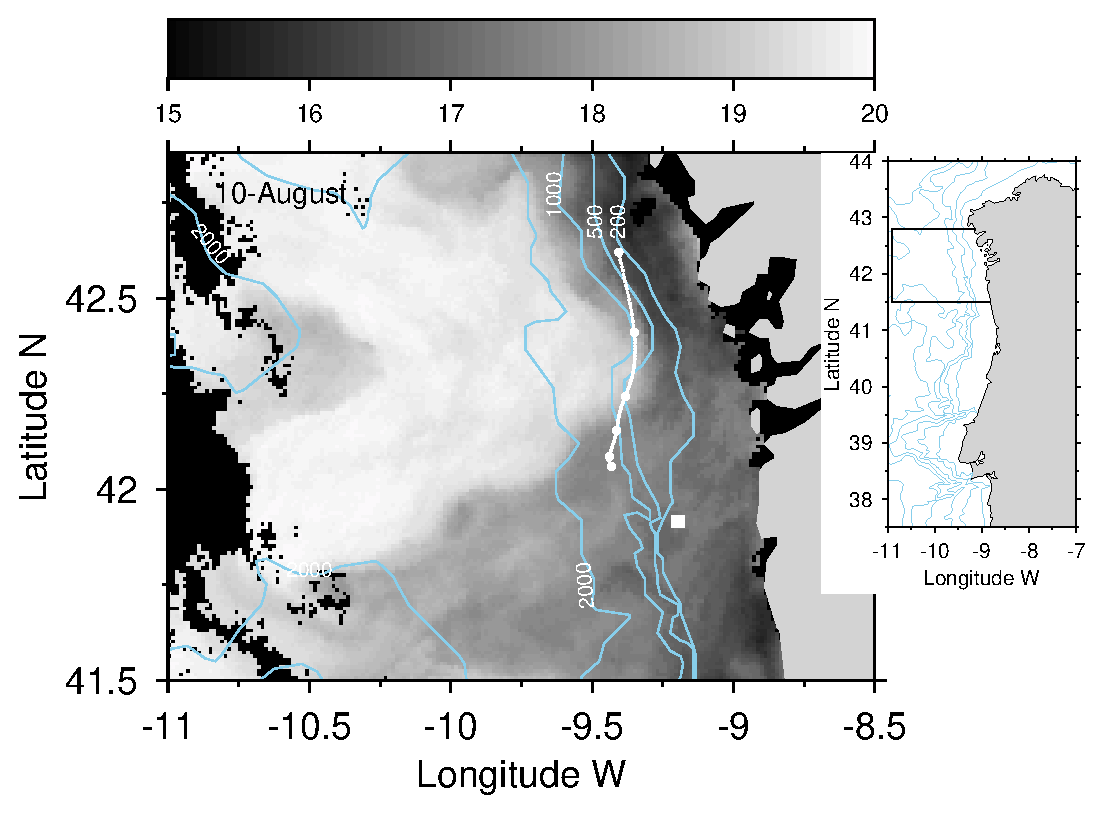
\includegraphics[width=9cm]{fig01}%
\caption{Drifter track (dotted line) and the position of the time
series observations (white square) of Leg 1 (2-10 August 1988)
overlaid on the sea surface temperature image of 10 August. Colder
upwelled waters are seen along the coast and extending offshore in
the filament south of 42\deg N. The drifter was always inshore of
the upwelling front, which receded towards
the coast during the observations. Isobaths are shown in metres.}%
\label{fig:cd114leg1}%
\end{figure}

The physical sampling strategy on board RRS Charles Darwin cruise
114 was designed to support Lagrangian primary production
experiments during Leg 1 (2-10 August 1998) on the shelf
(Fig.~\ref{fig:cd114leg1}) and Leg 2 (11-20 August) in the
filament (Fig.~\ref{fig:cd114leg2}). Further physical observations
were made following the drift experiments, at a time series
station on the shelf and in a spatial survey of the filament
structure. In the shelf experiment the work was based around the
drift of a primary production rig, while in the filament a primary
production rig and recoverable Argos buoy were deployed at the
centre of a cluster of 4 Argos drifters.   The rig and their water
tracking characteristics are detailed by \citet{Joint01}. It
comprised a small surface float, with radar reflector and radio
beacon, designed to offer minimum windage. A semi-submerged toroid
buoy, 1.2m in diameter was attached to the float and 3 sediment
traps at 30m, 40m and 50m acted as drogues. The drifter deployment
positions for the filament experiment (Fig.~\ref{fig:cd114leg2}b)
on 14 August were chosen on the basis of SST images transmitted to
the ship during previous days. Horizon Marine drifters released in
a 5nm side square in the core of the upwelling filament were
equipped with cylindrical 'holey sock' drogues (7m length, 1.2m of
diameter) at a nominal depth of 15m. The drifters had an
approximate drag area ratio of 50 which restricts wind slippage to
less than 1\velc\, for winds of 10\vel\, \citep{Niiler95}. They
were tracked with the ARGOS system, yielding 6-8 fixes per day.
\begin{figure} \centering %
\arribacap
\subfigure[]{
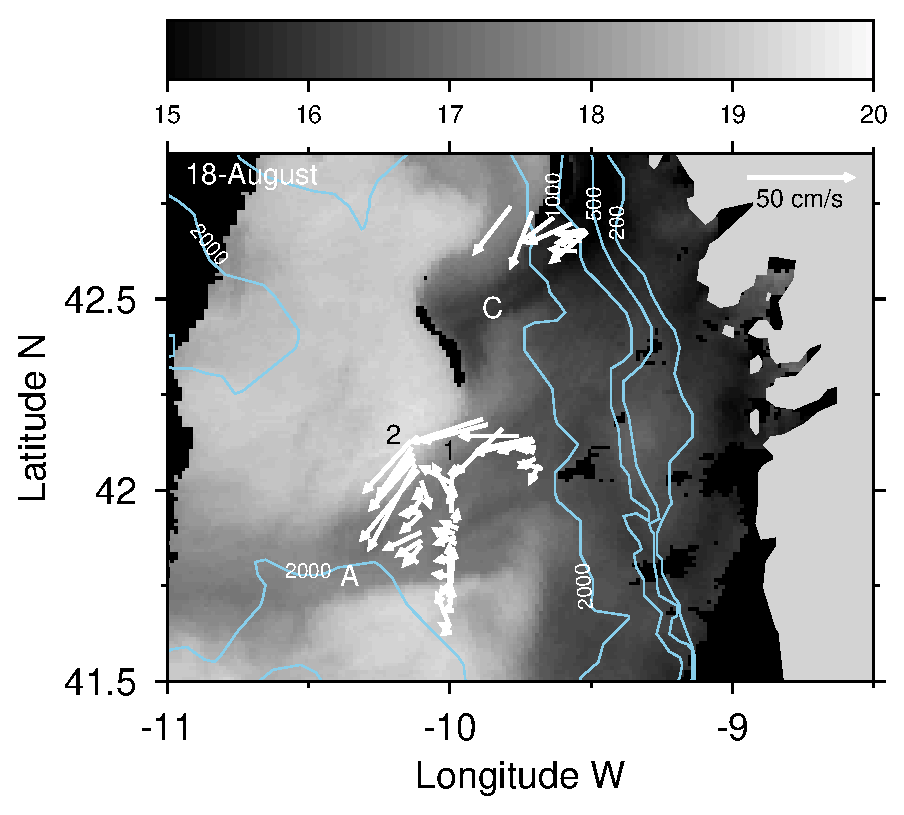
\includegraphics[width=7cm]{fig02a}}%
\subfigure[]{
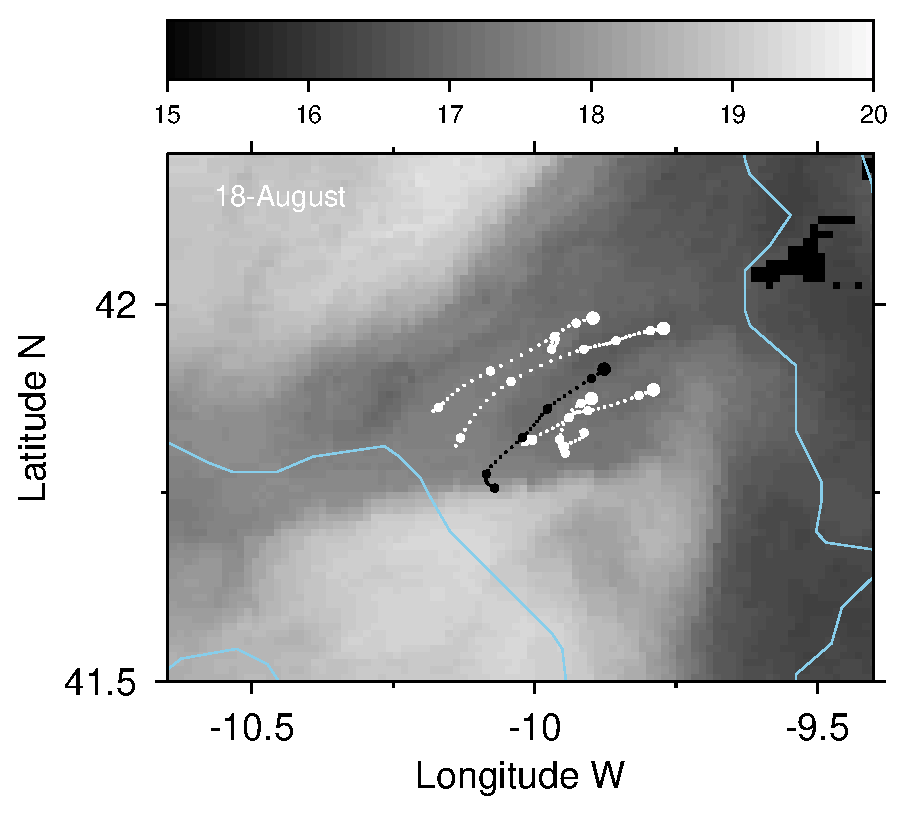
\includegraphics[width=7cm]{fig02b}}%
\caption{(a) Absolute ADCP velocities at 25m along sections during
Leg 2 (12-22 August 1988) overlaid on the sea surface temperature
image of 18 August. Colder upwelled waters extend from the coast
beyond the shelf break and offshore in filament B south of 42\deg
N. A newly developing filament C is seen near 42.5\deg N. Isobaths
are shown in metres. (b) Drifter tracks from 14 to 19 August
superimposed on blow up of SST image of (a). Large dots mark the
release point and smaller dots start of each
day. The instrument rig track is shown in black. The isobath shown is 2000 m.}%
\label{fig:cd114leg2}%
\end{figure}
The same sampling set up as in cruise CD105, described in
Chapter~\ref{ch:spring}, was used again in CD114. The CTD salinity
data were calibrated against 8 (leg A) and 11 (leg B) water
samples analysed on a Guildline Autosal bench salinometer. A
constant offset of 0.042$\pm$0.008psu (0.029$\pm$0.006psu)  was
found for leg A (leg B). CTD temperatures agreed well with
calibrated digital reversing thermometers and no correction was
applied.

CTD casts were made during both legs of the cruise adjacent to the
primary production rig approximately every 6 hours. Additionally,
casts were made across the base of the 42\deg N filament and on
other short sections, totalling 83 casts over the cruise. Velocity
profiles along the ship track were obtained with the RD
Instruments hull-mounted 153.6kHz narrow-band ADCP already
described in Chapter~\ref{ch:spring}. The complete Acoustic
Doppler Current Profiler data set and in-depth details of
processing are given by \citet{Torres99} and follow the steps
described in Chapter~\ref{ch:spring}. Bin size was set at 8m and
data from above 25m were rejected as unreliable. ADCP data were
recorded in 5 min ensembles during Phase 1, and in 2 min ensembles
during Phase 2. The overall quality of Leg 1 data was good, with a
typical depth range of 300m or to the sea bed on the continental
shelf.  Leg 2 data, recorded in 5 min ensemble averages, were of
poorer quality with penetration typically to only 150 m.
\begin{figure}
\centering \hspace*{-.5cm}\subfigure[]{
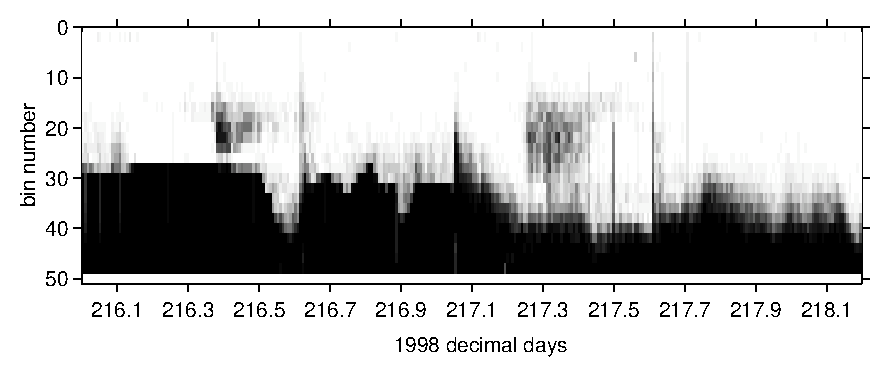
\includegraphics[width=9cm,trim=0 20 0 2,clip]{pgoodleg1}}\\
\subfigure[]{
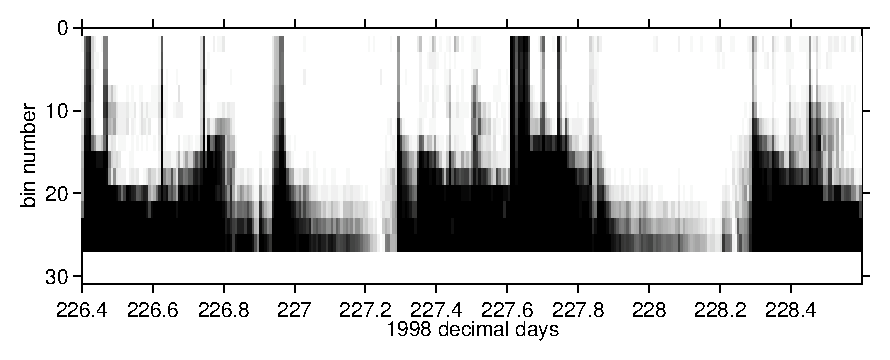
\includegraphics[width=9cm,trim=0 8 5 5,clip]{pgoodleg2}
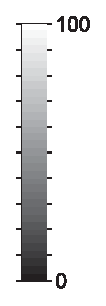
\includegraphics[height=3.5cm,trim=0 -5 0 0,clip]{palette}}
\caption{Example of Percentage-good pings vs. time and bin number
for a) Leg 1 and b) Leg 2 for the 150Khz NB ADCP.}
\label{fig:cd114pg}
\end{figure}

A subset of the Percentage good (PG) record for Leg 1 and 2
exemplifies the differences encountered during both legs
(Fig.~\ref{fig:cd114pg}). Good quality data were obtained during
Leg 1 (Fig.~\ref{fig:cd114pg}a), with PG in excess of 85\% in the
water column, sharply decreasing to zero at the bottom (black in
the example). During Leg 2 (Fig.~\ref{fig:cd114pg}b), PG in the
top water column was similar to Leg 1, but penetration was much
more limited, at most 200m when on station. The penetration was
greatly reduced at times of sailing against the prevailing sea
when it was impossible to record below 50m or less (e.g. day 227.6
in Fig.~\ref{fig:cd114pg}b). The physical installation of the
transducer is believed to account for much of its malfunctioning
as bubbles are trapped beneath the ship's hull \citep{New92}.
These problems were particularly evident during Leg 2 where the
decrease in passive acoustic reflectors worsened the ADCP
performance. This is supported by the rapid decreased of the
Amplitude Gain in Leg 2, when, on average, it fell below 50 at
100m while in Leg 1, it reached 50 at 200m.

\begin{figure}
\centering \subfigure[]{
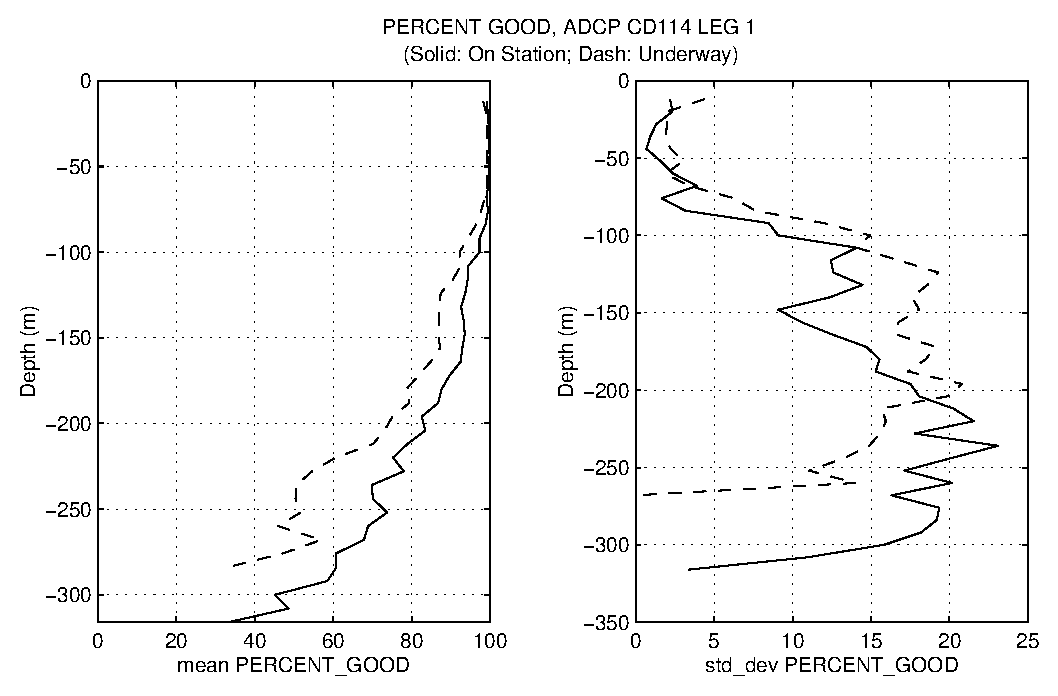
\includegraphics[width=9cm]{quality1}}\\
\subfigure[]{
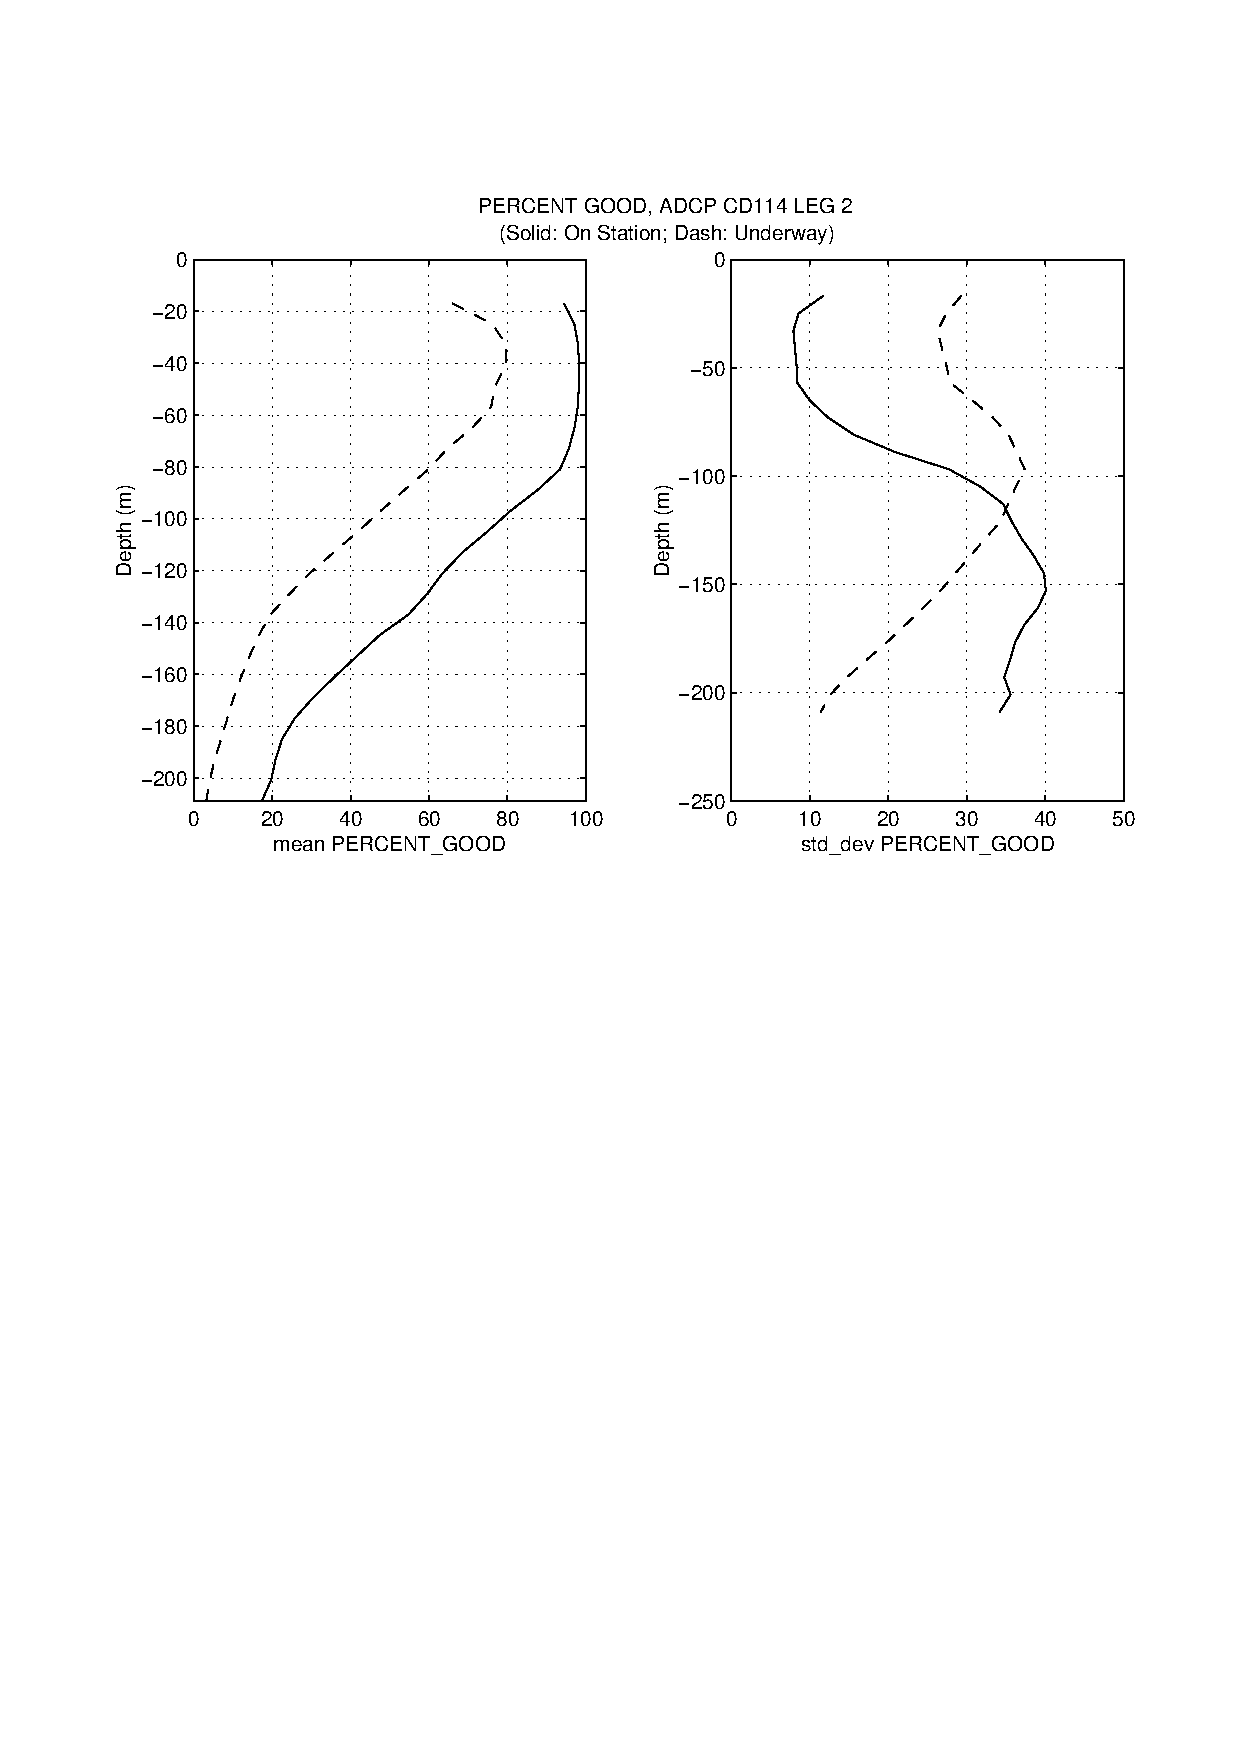
\includegraphics[width=9cm]{qualitypgleg2}}
\caption{Comparison between underway and on station averaged and
standard deviation profiles of Percentage Good for a) Leg 1 and b)
Leg 2.} \label{fig:cd114quality}
\end{figure}

The data quality was further assessed by comparing underway and on
station profile averages. The PG profile averages summarise the
main differences between the two legs seen in all other variables
checked (Fig.~\ref{fig:cd114quality}). Underway and on station
mean and standard deviation profiles showed relatively small
differences during Leg 1 (Fig.~\ref{fig:cd114quality}a),
negligible in the top 100m and less than 10\% below to 200m,
increasing downwards. Differences less than 5\% were found in the
standard deviation with absolute values less than 20\%. It was
small ($<$5\%) in the top 70-80m, but increased rapidly reaching
10-20\% below 100m. During Leg 2 (Fig.~\ref{fig:cd114quality}b), a
consistent 20\% difference in the mean and standard deviation was
evident between underway and on station data through the water
column. Mean values decreased rapidly below 80m while on station
(60m while underway), on average yielding unreliable data from
140-150m. The standard deviation values were larger during Leg 2,
but its change with depth was similar to Leg 1.

The ADCP was checked for misalignment of the transducer with
respect to the gyro compass by calibrating the data. In
conjunction with the water method described in
Chapter~\ref{ch:spring}, the bottom track method was attempted for
Leg 1, which compares acceleration relative to the water and over
the ground as measured with the ADCP only.
\begin{table}
  \centering
\begin{tabular}{cccc}
\hline \hline & \multicolumn{2}{c}{Leg 1} & Leg 2 \\ \hline &
\multicolumn{1}{c}{Bottom Track} & \multicolumn{1}{c}{Water
Track} & \multicolumn{1}{c}{Bottom Track}\\
$\beta \, \pm \, \sigma$ & 1.01 $\pm 0.01$ & 1.02 $\pm 0.01$ &
 1.04 $\pm 0.02$ \\
$\alpha \, \pm \, \sigma$ & -0.1 $\pm 0.6$ & -0.1 $\pm 1.0$ &
0.4 $\pm 1.0$\\
\hline \hline
\end{tabular}
  \caption{Calibration parameters for CD114}\label{tb:cd114cal}
\end{table}
The values obtained for amplitude and angle with their respective
standard deviations for all calibrations attempted are shown in
Table~\ref{tb:cd114cal}.  The calibration parameters during the
Leg 1 agree very well for water and bottom track estimates
although they differ with respect to the phase estimate of Leg 2.
However, due to the poorer quality of the data during the last Leg
only the calibration coefficients for Leg 1 were considered. Their
small value suggested that no correction of the data was needed.

Direct observations of turbulent kinetic energy dissipation
$\epsilon$ were made at a 1 cm resolution with the Free-falling
Light Yo-yo (FLY) shear microstructure profiler (see
\citet{Dewey87}). A description of the instrument and data
processing is detailed in Appendix~\ref{ap:fly}. During the six
day Lagrangian productivity drifter experiment on the shelf (Leg
1, Phase 1), groups of dissipation profiles were made
approximately every 6 hours.  Each group, or series, contained
about 10 profiles.  Leg 1, Phase 2 comprised an Eulerian internal
wave experiment lasting $\sim$24 hours at a location 5km shoreward
of the shelf break in about 170m (Fig.~\ref{fig:cd114leg1}).  FLY
profiled the water column with a repeat cycle of $\sim$6 min with
breaks of 20 to 30 minutes every 3 to 4 hours for battery
recharging. A more in depth description of the data can be found
in \citet{Barton01}. During Leg 2, the filament was sampled with
the FLY probe, CTD and shipborne ADCP. As the drifter array moved
away from the coast, partial across-filament transects were
performed. These were interspersed every 6 hours with biology
stations conducted next to the primary production buoy. The
detailed spatial sampling of the filament was undertaken with the
FLY in $\sim$10 min cycles of 3-5 profiles to an average depth of
250 m. Calculation of the rate of turbulent kinetic energy (TKE)
dissipation from the FLY shear microstructure data followed
\citet{Dewey87} and \citet{Inall98} and is described in the
Appendix \ref{ap:fly}. TKE data were converted to vertical
diffusion coefficient, $K_z$, using $K_z=0.2\epsilon /\rho N^2$
\citep{Osborn80}, where N is the local buoyancy frequency; and
$\rho$ is density (assuming that $\epsilon$ is in
$\mathrm{Wm^{-3}}$). FLY temperature and conductivity records were
calibrated against the calibrated CTD data.
\section{Results}
\subsection{Background and evolution}
\begin{figure}
\centering %
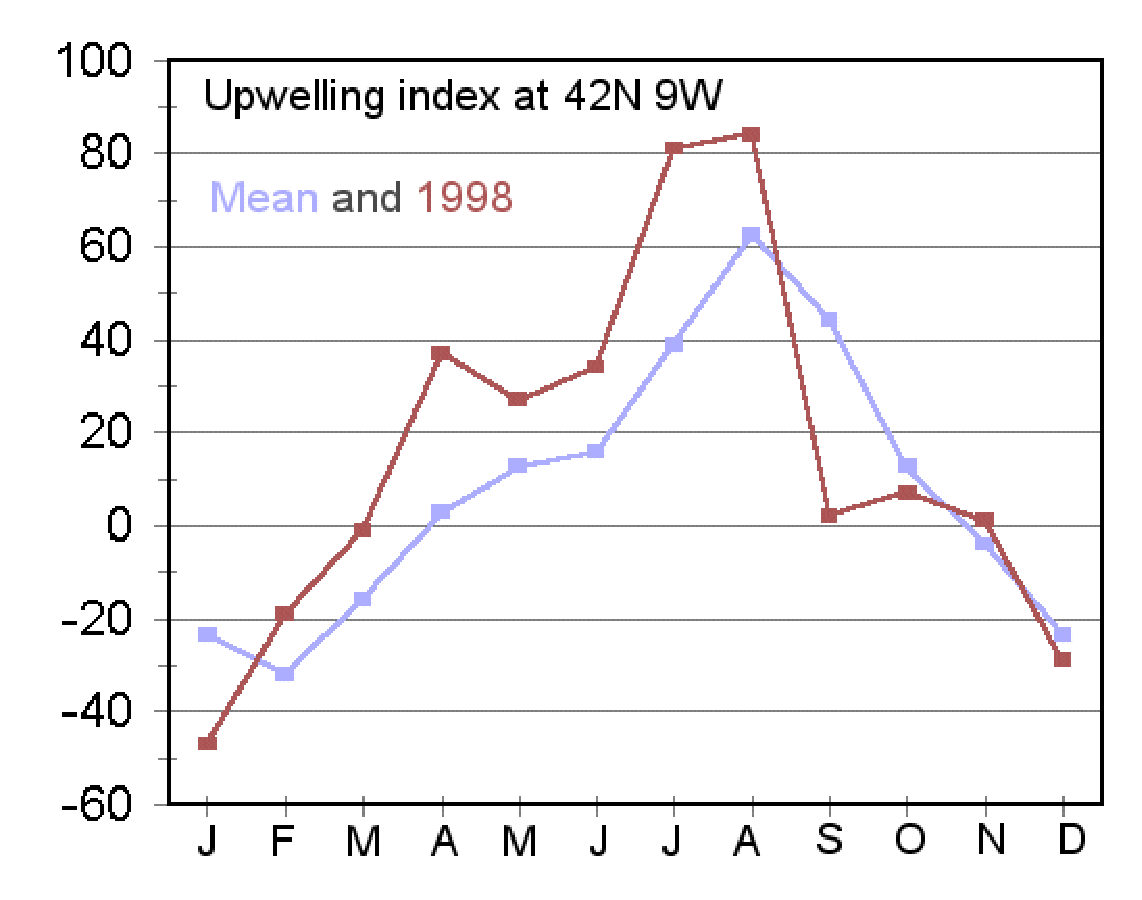
\includegraphics[width=8cm]{upwidx98}%
\caption{Monthly averages of Upwelling index calculated for a cell
centred at 42\deg N 9\deg W from daily ECWNF winds for years
1986-1998 (blue) and 1998 (red).}
\label{fig:cd114upidx}%
\end{figure}
The seasonal cycle in the wind is clear in the interannual mean of
derived Ekman transport (Fig.~\ref{fig:cd114upidx}). In 1998
(Fig.~\ref{fig:cd114upidx}), wind became upwelling favourable in
April, earlier than in the average year, and was stronger than
average until it reached a peak in August. Wind strength dropped
quickly in September to weaker than average values, but remained
weakly upwelling favourable until December. In AVHRR images a band
of cold upwelled water was clearly visible next to the coast after
12 June 1998 (Fig.~\ref{fig:cd114sst}a). The upwelling front
quickly developed short scale instabilities like the ones
described by \citet{Haynes93}.
\begin{figure}
\centering \abajocap%
\subfigure[12 June]{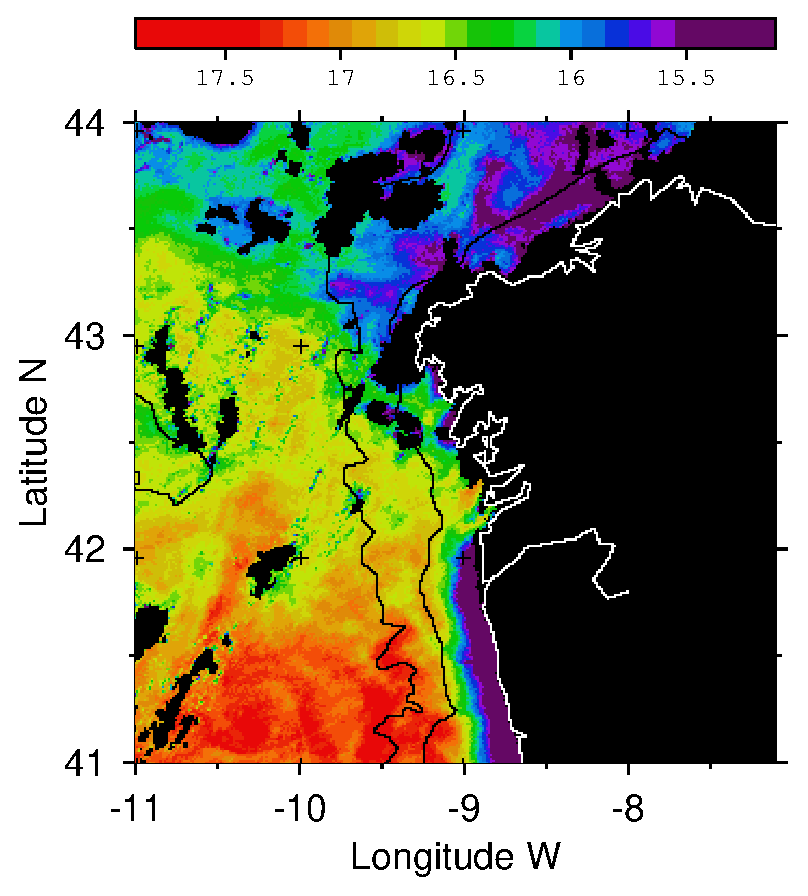
\includegraphics[width=5cm]{12jun980401gasstpcol}}%
\subfigure[29 June]{\includegraphics[width=5cm]{29jun981741gasstpcol}}%
\subfigure[8 July
]{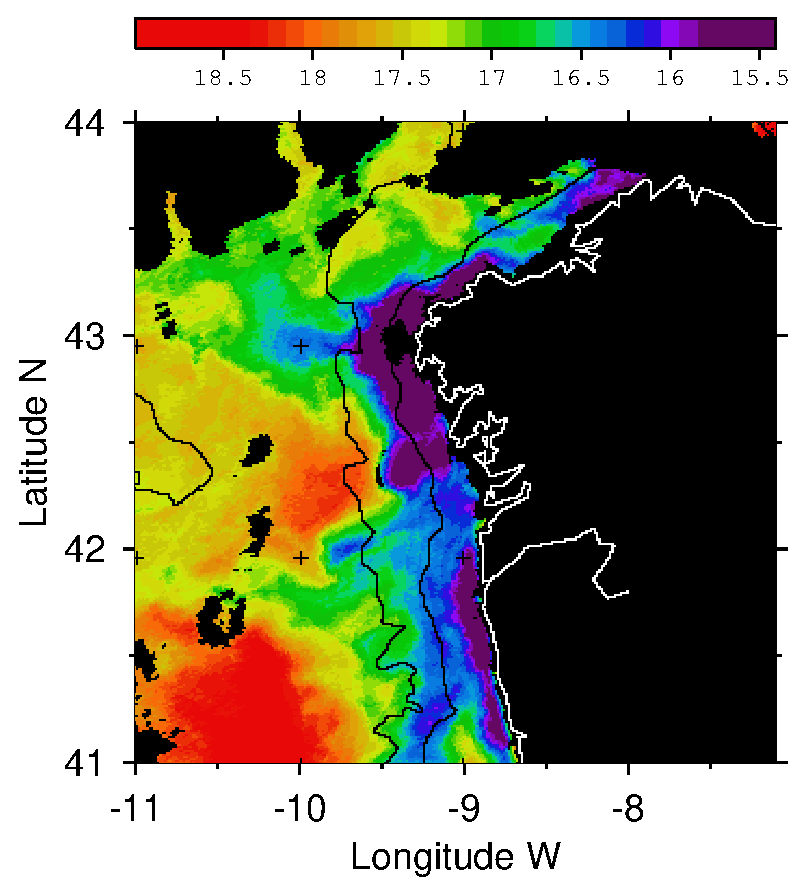
\includegraphics[width=5cm]{08jul981409gasstpcol}}\quad
\subfigure[15 July]{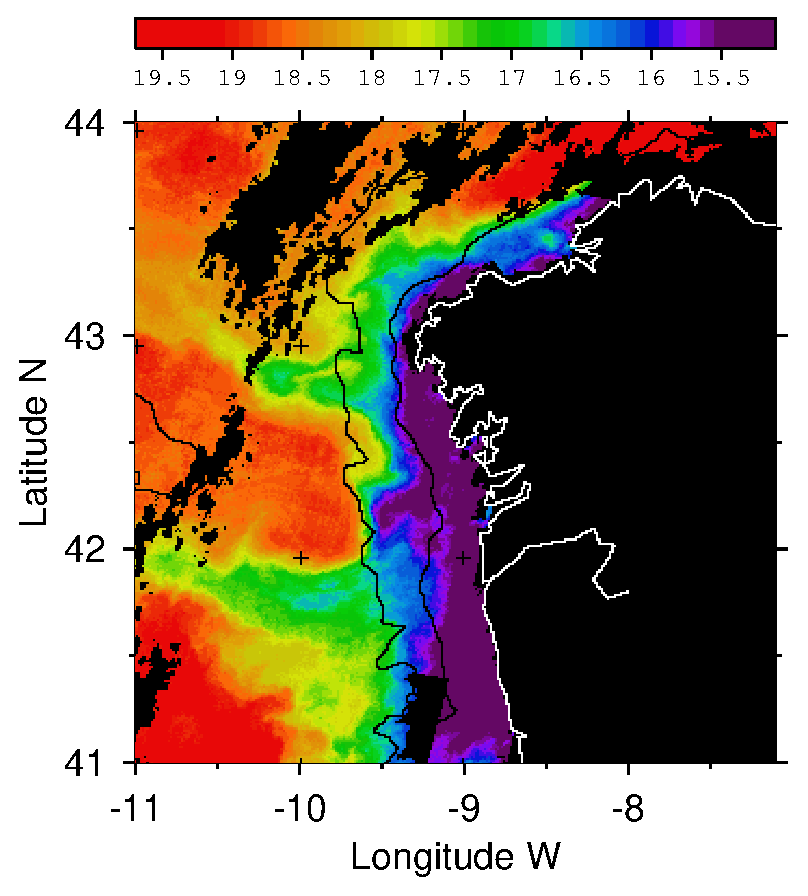
\includegraphics[width=5cm]{15jul980659gasstpcol}}%
\subfigure[29 July]{\includegraphics[width=5cm]{29jul981519gasstpcol}}%
\subfigure[3 August
]{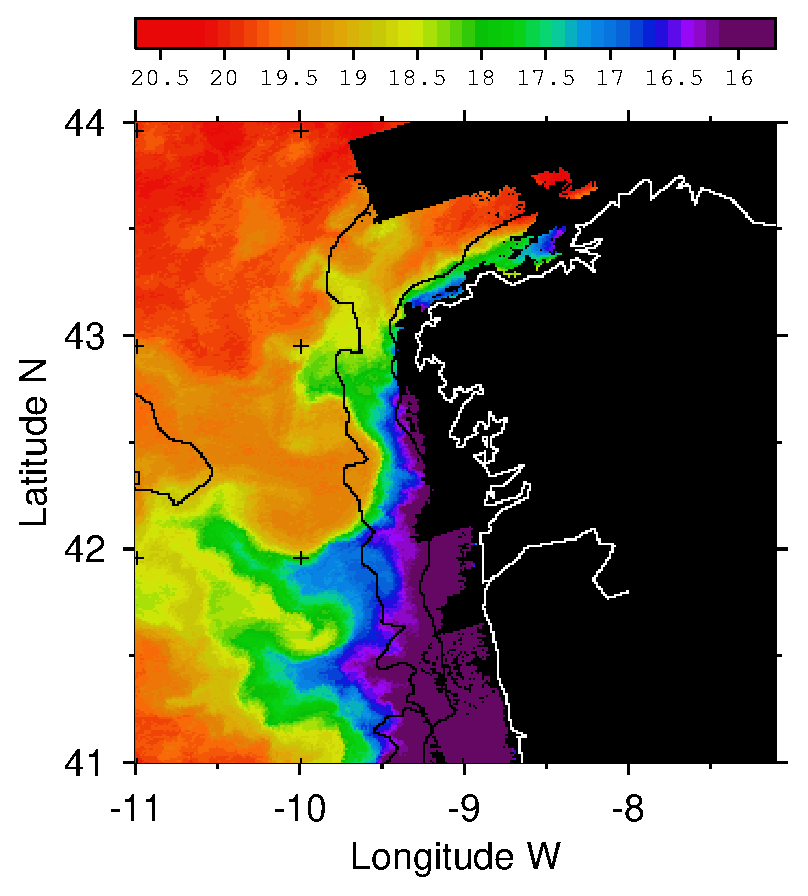
\includegraphics[width=5cm]{03aug981423gasstpcol}}\quad
\subfigure[10 August]{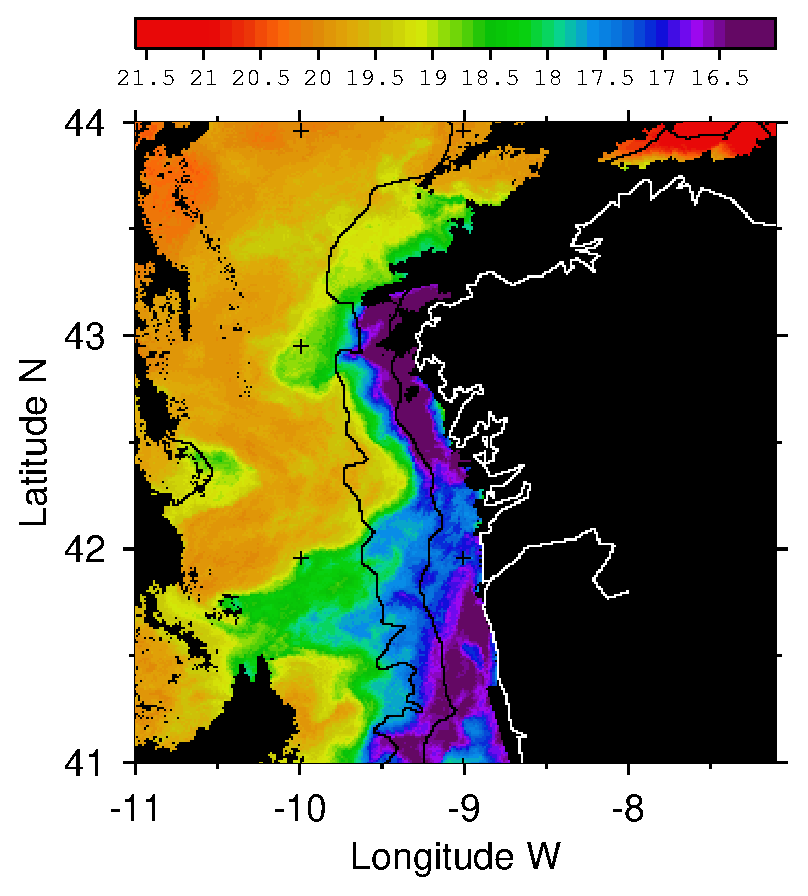
\includegraphics[width=5cm]{10aug981446gasstpcol}}%
\subfigure[5 September]{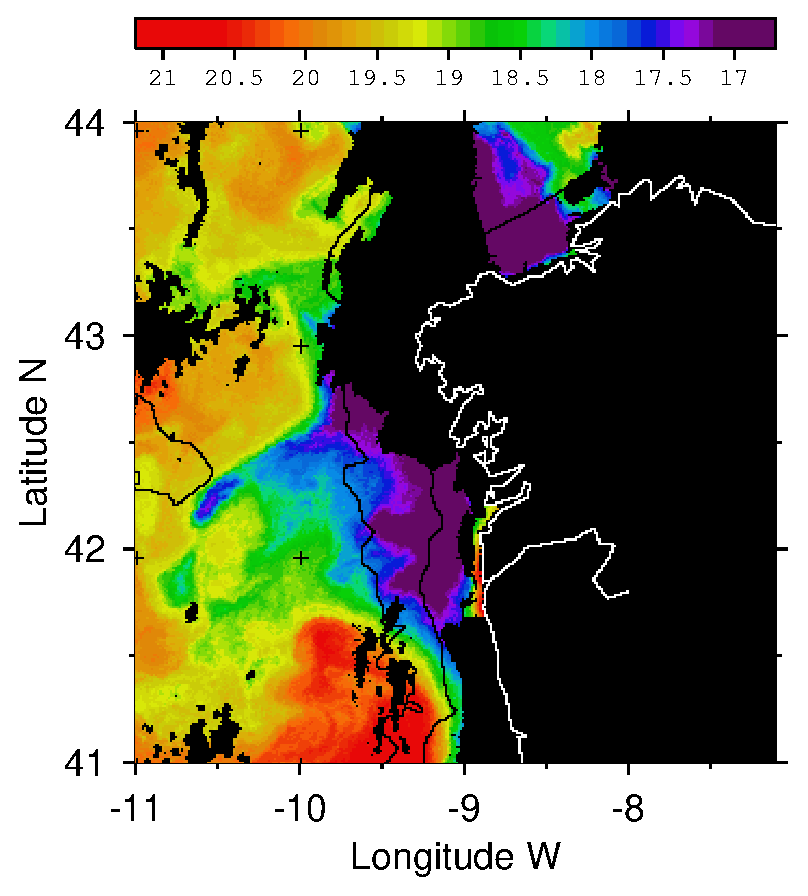
\includegraphics[width=5cm]{05sep981500gasstpcol}}%
\subfigure[15 September
]{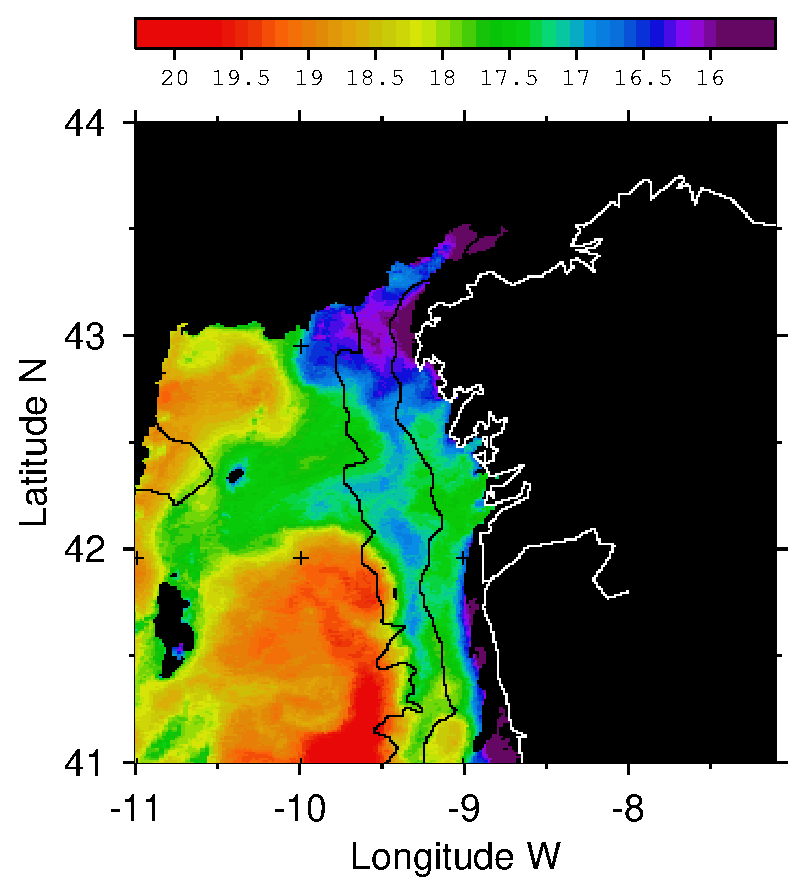
\includegraphics[width=5cm]{15sep980314gasstpcol}}\quad
\caption{SST images during the upwelling season of 1998 depicting
some of the characteristics of the season evolutions. Note the
different scales on each image in order to highlight frontal
areas. } \label{fig:cd114sst}
\end{figure}
The sustained northerly winds drove the upwelling front steadily
offshore until the upwelled water expanded across the 200m isobath
late in June (Fig.~\ref{fig:cd114sst}b), at which time the first
filament-like structure developed off Cape Finisterre. By 8 July
(Fig.~\ref{fig:cd114sst}c), two filaments, one at 42\deg N and one
at Cape Finisterre were fully developed. The 42\deg N filament
(Filament A after \citet{Smyth01}) was detectable until the end of
the upwelling season (late September) while the Finisterre
filament disappeared in mid-July when the band of upwelled water
receded in the north and became wider south of 42\deg N
(Fig.~\ref{fig:cd114sst}d-e). During the cruise, winds were
generally upwelling favourable in direction but went through
several cycles of relaxation and strengthening
(Fig.~\ref{fig:cd114winds}).  On 31 July, prior to Leg 1, winds
were strong ($\sim$15\vel) towards the southwest, became more
southward and weaker (5-10\vel) during 2-5 August, and then
weakened to near zero at the end of the shelf drift experiment and
during the internal wave observations on 8-9 August. Strong
southward winds prevailed for the first days of the Leg 2 filament
experiment but weakened from 10\vel on 13 August to near zero on
16 August, when the first filament section was completed. Winds of
$\sim$10\vel\, were re-established for the second filament section
on 17-18 August and persisted until the end of the cruise. The
42\deg N filament A was present throughout, although it diminished
in response to weakening winds and reactivated with the renewal of
upwelling favourable winds. At the start of the cruise in early
August upwelling immediately south of Cape Finisterre weakened and
another filament (Filament B after \citet{Smyth01}) north of
41\deg N developed (Fig.~\ref{fig:cd114sst}e). Filament B moved
north (Fig.~\ref{fig:cd114sst}f) and merged with filament A by 10
August (Fig.~\ref{fig:cd114sst}g), at the end of the first wind
relaxation. With the re-establishment of strong winds by 12 August
the band of coastal upwelling widened and filament definition in
the SST images strengthened. \arribacap
\begin{figure}
\centering %
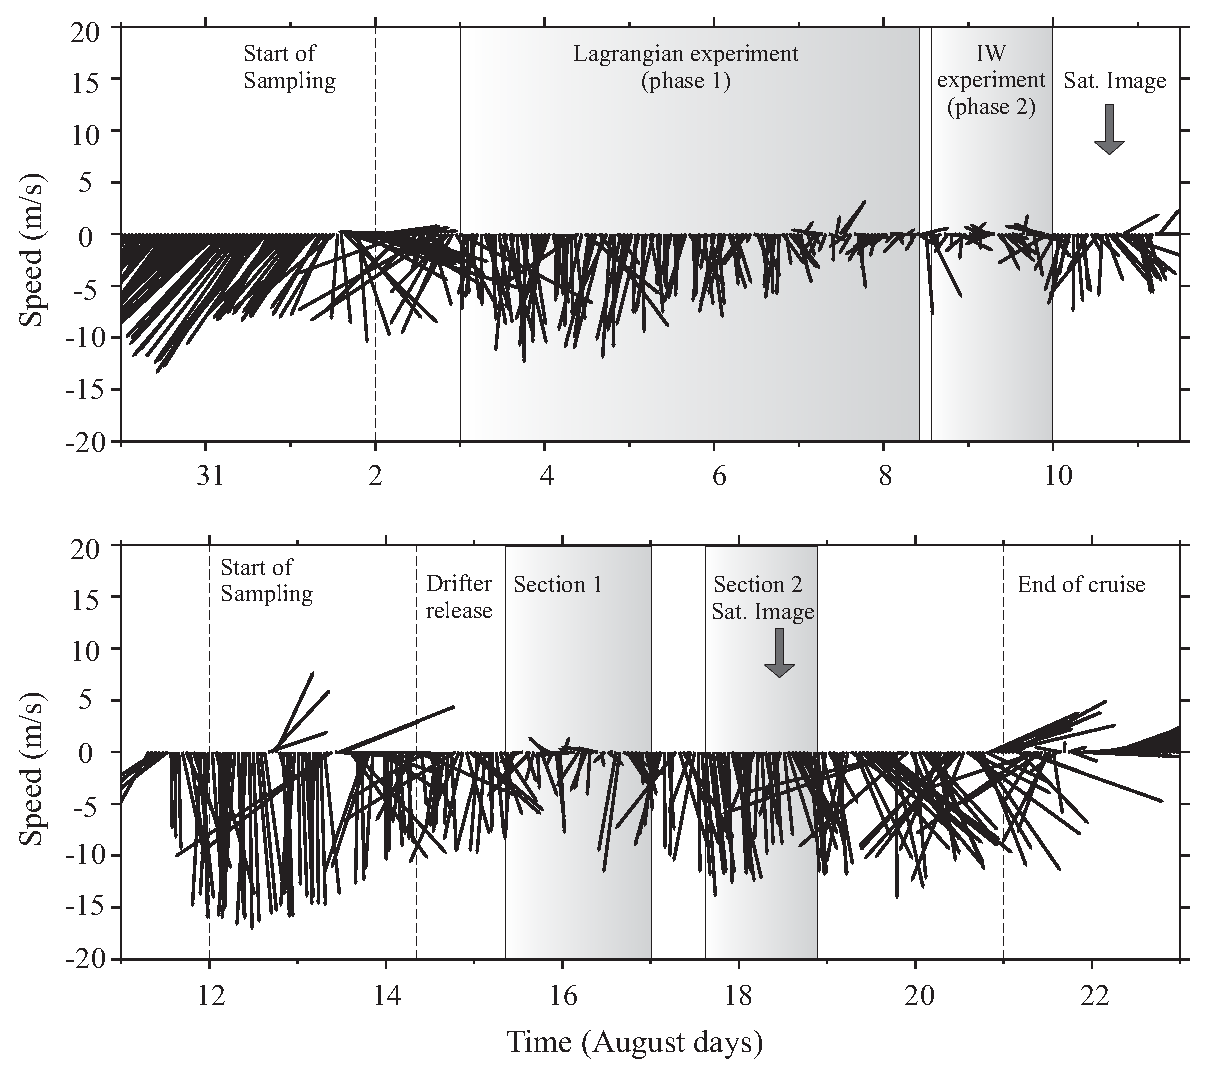
\includegraphics[width=10cm]{windall}%
\caption{Wind vector series for Leg 1 (upper) and Leg 2 (lower).
Southward wind vectors point vertically down the page.
Timing of the different experiments is shown.}%
\label{fig:cd114winds}%
\end{figure}
Subsequent wind relaxation was evident in later images as a
narrowing and weakening of filament A. It was 30km wide and over
200km long at the time of the spatial sampling. The final stages
of the filament during September coincided with slackening in the
winds as reflected by the monthly average upwelling index. The
offshore extend of the coastal upwelling band south of the
filament narrowed (Figs.~\ref{fig:cd114sst}h-i). The filament
widened and was advected northwards while a warm tongue developed
offshore of the upwelling front.
\subsection{The Shelf experiment Leg 1}
\subsubsection{Water column structure and fluxes during the drift}
\begin{figure}
\centering %
\subfigure[]{
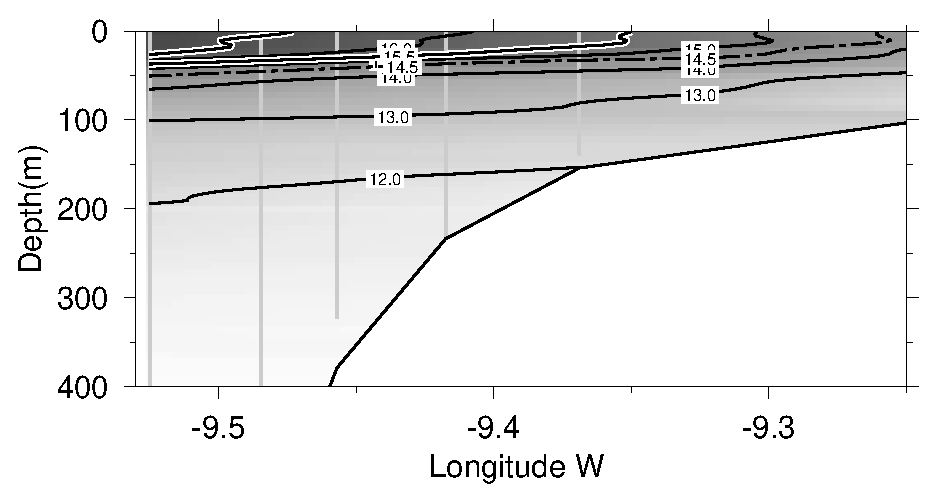
\includegraphics[width=10cm]{shelftranT}}\\
\subfigure[]{
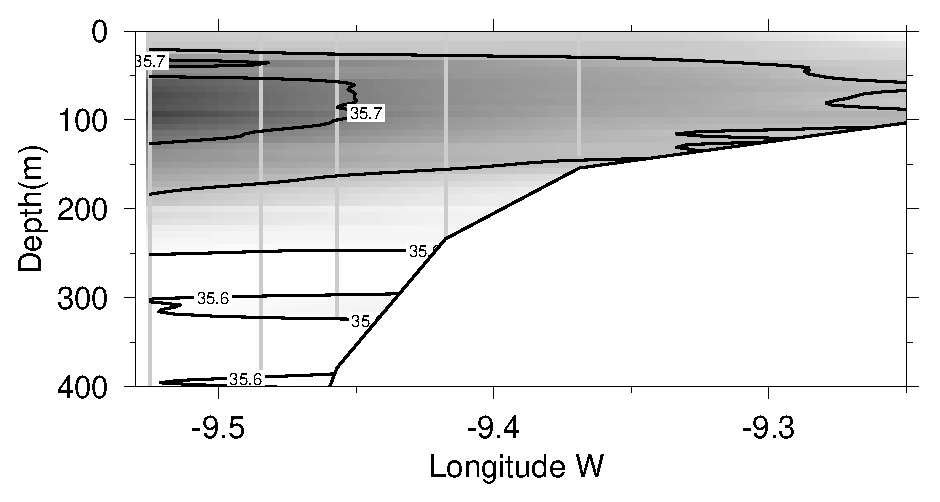
\includegraphics[width=10cm]{shelftranS}}\\
\subfigure[]{
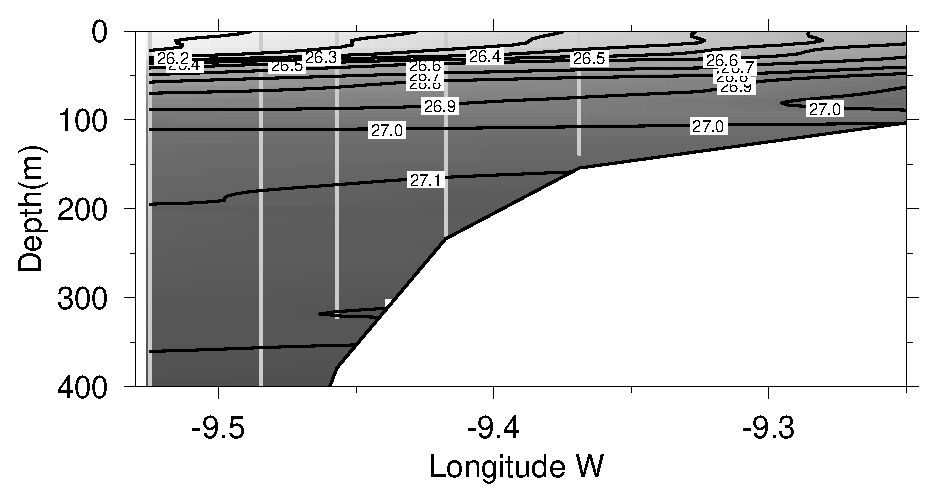
\includegraphics[width=10cm]{shelftranD}}\\
\caption{(a) Temperature (b) Salinity and (c) Density in the
across-shelf transect at the beginning of CD114 cruise.}
\label{fig:cd114_shelftran}%
\end{figure}
At the start of the cruise, a cross-shelf transect at 42.6\deg N
latitude was undertaken to determine the best position for the
drift experiment (Fig.~\ref{fig:cd114_shelftran}). An across-shelf
temperature gradient (2\deg C in 23km) was present in the top 50m
of the water column. Isotherms and isopycnals all showed an
uplifting onshore, indicative of coastal upwelling, with a
vertical displacement of $\sim$50m across the section at 100m
depth. The slope of the isolines decreased with depth but was
still evident at 200m and below (Fig.~\ref{fig:cd114_shelftran}c).
The salinity displayed a broad salinity maximum off the shelf,
larger than 35.7psu between 50 and 200m depth, which became
narrower and less saline onshore
(Fig.~\ref{fig:cd114_shelftran}c). The productivity rig was
released at 9.4\deg W in 150m of depth.
\begin{figure}[th]
\centering %
\subfigure[]{
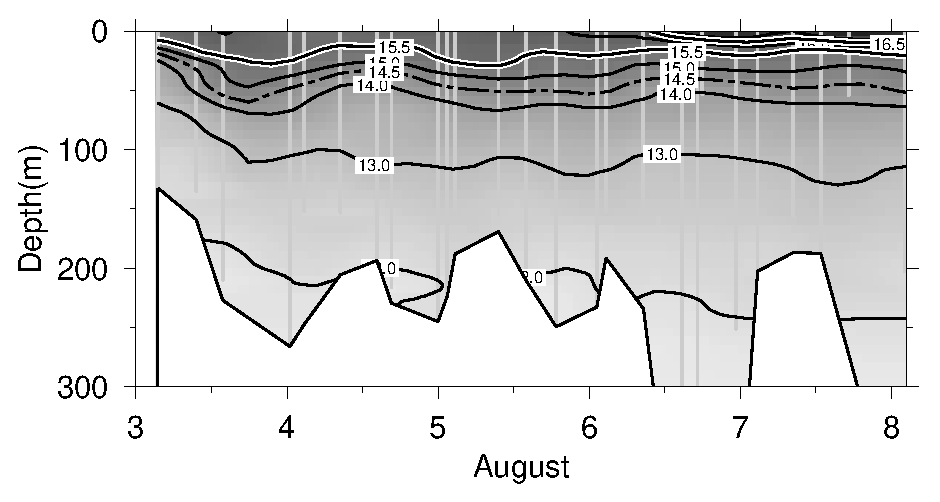
\includegraphics[width=10cm]{driftaT}}\\
\subfigure[]{
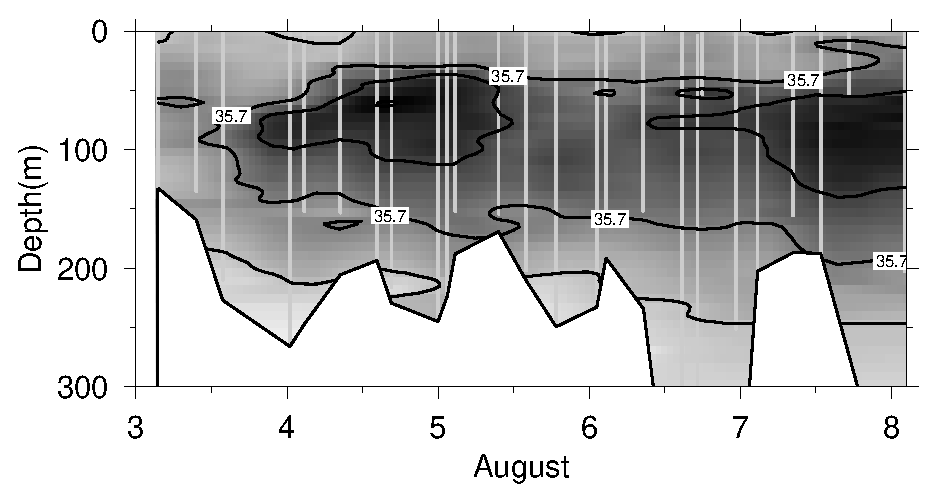
\includegraphics[width=10cm]{driftaS}}\\
\subfigure[]{
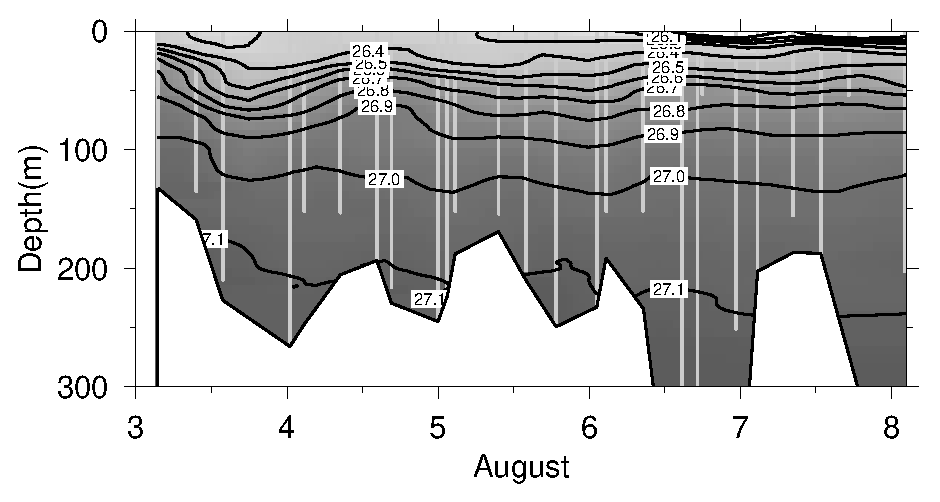
\includegraphics[width=10cm]{driftaD}}\\
\caption{(a) Temperature (b) Salinity and (c) Density during the
shelf drift experiment. The buoy gradually moved into
deeper water.}%
\label{fig:cd114_drifta}%
\end{figure}
As the wind relaxed during the Phase 1 drift experiment the
internal water column structure remained essentially unchanged,
which suggested that the buoy remained within a single
near-surface water packet (Fig.~\ref{fig:cd114_drifta}). The main
features were the downward slope of the isotherms over the first
$\sim$24h, changes in the high salinity core at $\sim$75m and
warming of the upper few tens of metres towards the end of the
drift experiment. The downward slope in the isolines on the first
day corresponded to rapid offshore drift into deeper waters. It
was the least ``truly Lagrangian'' stage overall, considering the
strong velocity shear of the top 60m
(Fig.~\ref{fig:cd114adcpleg1}). The range of salinity on the 26.9
isopycnal, located approximately at 80m depth, was less than
0.1psu. The data seen in T/S space conformed with the expected
variability of \enawt at these positions. The drifter moved into
deeper waters during the last two days, and the daily mean surface
temperature increased by $\sim$1.5\deg C as the surface layers
stratified in near zero wind (Fig.~\ref{fig:cd114_drifta}a). This
increase occurred throughout the region \citep{Smyth01}. The
stratification reached maximum daily values after midday as
suggested by the short fluctuations of up to 1.5\deg C in the
underway surface temperature record caused by the pitching of the
ship.

\begin{figure}
\centering %
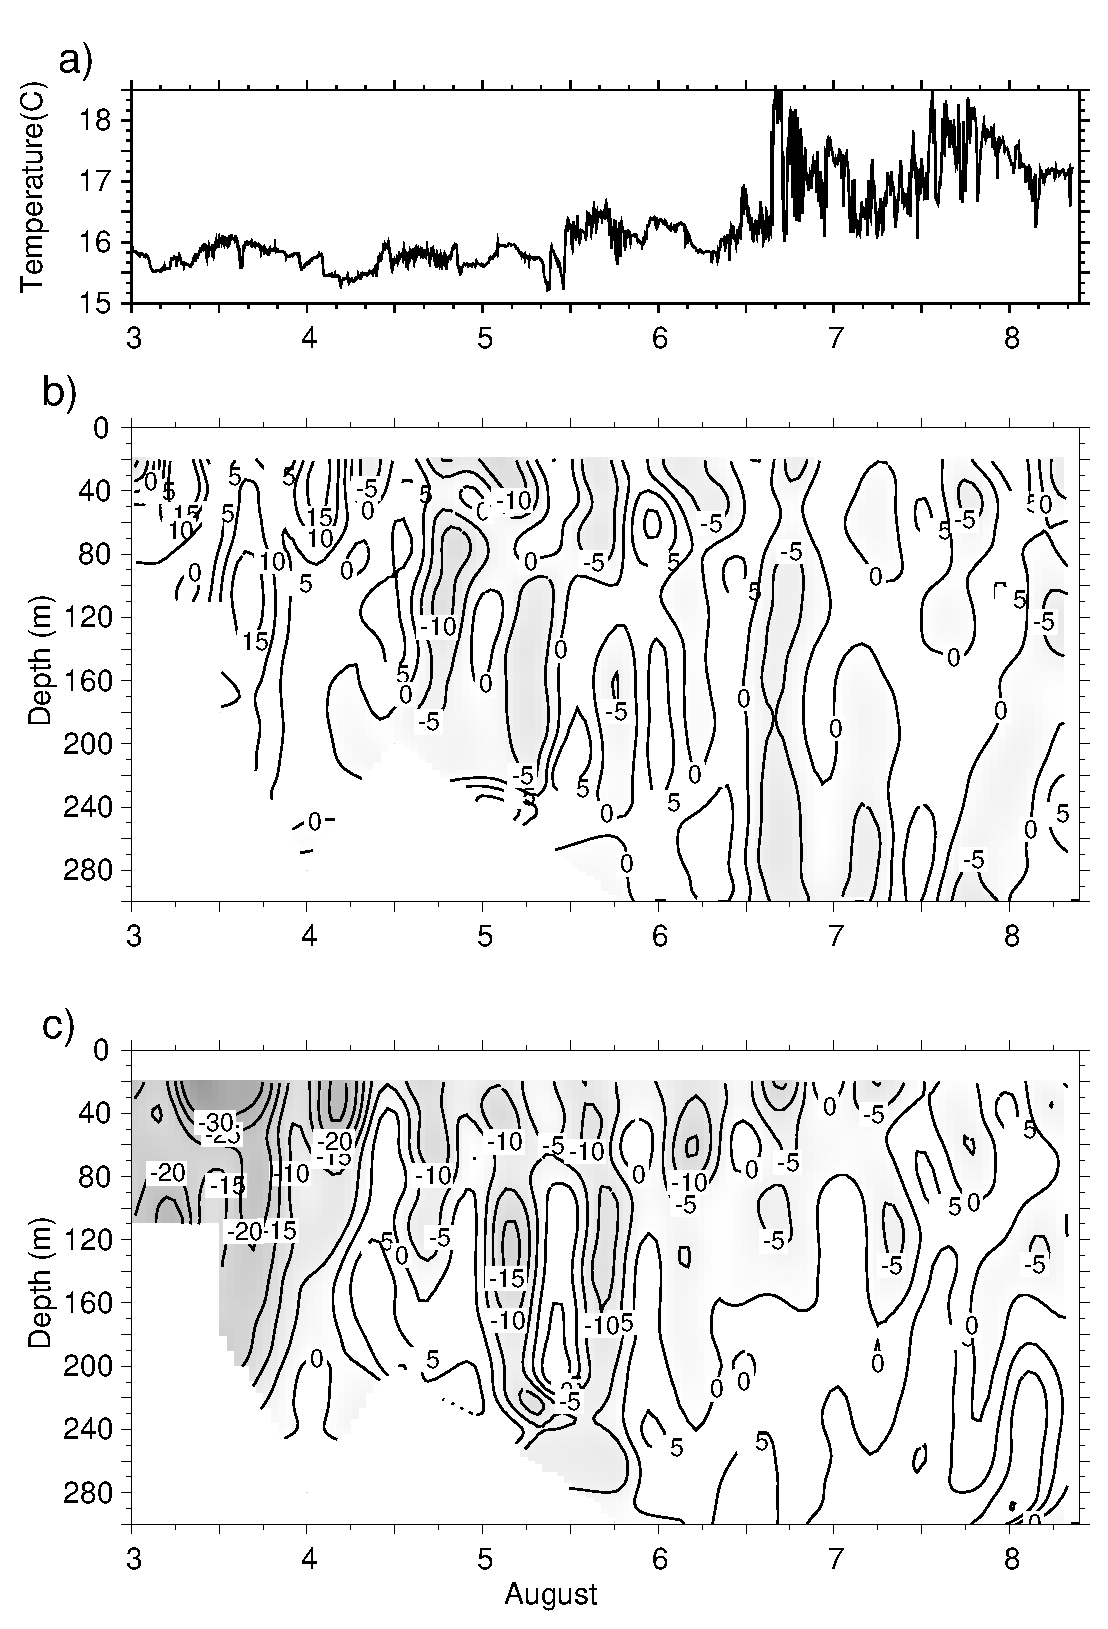
\includegraphics[width=12cm]{adcpleg1}%
\caption{(a) Surface temperature (b) east-west and (c) north-south
components of ADCP velocity during the shelf drift experiment. The
buoy gradually moved into
deeper water.}%
\label{fig:cd114adcpleg1}%
\end{figure}
Shipborne ADCP records made within 1.5km of the rig during its
drift show a change from initially relatively strong ($>$0.3\vel)
southward flow to weak ($<$0.1\vel) northward flow
(Fig.~\ref{fig:cd114adcpleg1}). The drift took place between neaps
(31 July) and springs (9 July). During the first day, a wind
driven surface jet with strong southward and weaker eastward flow
was apparent. On the next two days (4 and 5 August) the currents
were characterised by a return to tidally dominated flow (mainly
M2 tide), with some baroclinic structure evident (as expected for
a shelf edge). From 6 August, the tidal velocities weakened, which
was commensurate with drift out into deeper water. At the same
time there was an increase and shoaling of the northward
component, implying an increase in northward transport of water
throughout the entire water column measured. The east-west
component indicated predominantly shoreward flow in the first days
of the series, even though winds were still strongly upwelling
favourable and would be expected to correspond to offshore flow.
This apparent paradox of a net onshore flow component during
upwelling favourable wind can be resolved by considering the
volume fluxes in relation to the orientation of the bathymetry
(Fig.~\ref{fig:cd114fluxes}).
\begin{figure}
\centering %
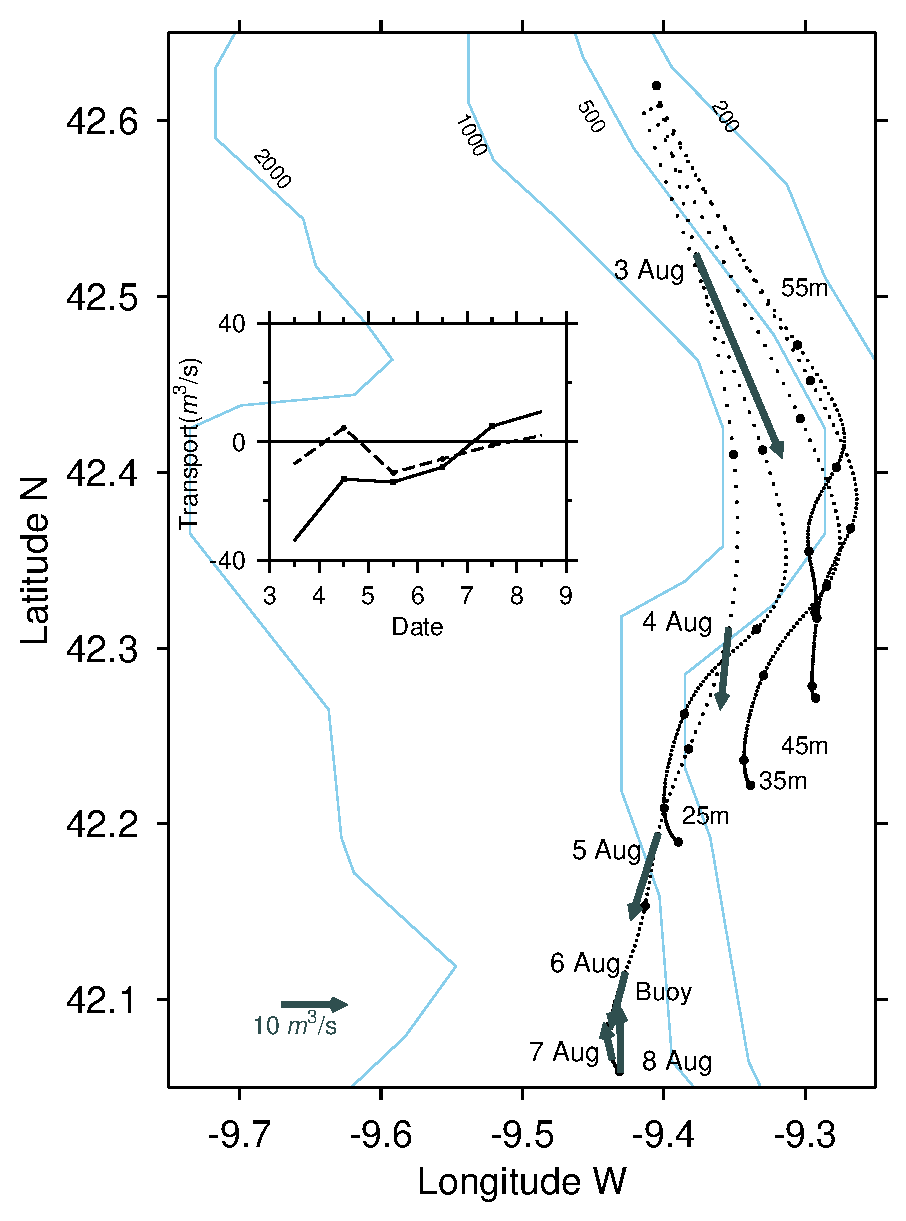
\includegraphics[width=8cm]{adcpflux}%
\caption{Smoothed track of the drift buoy and pseudo-trajectories
calculated from the ADCP observations during the shelf experiment,
showing the flow following the isobaths (indicated in m). The dots
mark each day beginning on 3 August. The black arrows indicate the
direction and strength of the integrated daily transport.  Shown
inset are the daily transport components across (dashed) and along
(solid line) local isobaths. Note the change from offshore
southward transport to onshore poleward.}
\label{fig:cd114fluxes}%
\end{figure}
The buoy trajectory and pseudo-trajectories calculated from the
ADCP data at different levels, all low pass filtered with a half
power point at 40 h, show the overall flow to follow broadly the
pattern of the isobaths.  Daily average depth-integrated eastward
and northward fluxes were calculated from the ADCP data and
extended to the surface with the drifter velocities.  When
superimposed on the buoy track each mid-day, the weakening and
reversal of the alongshore flux vectors with time is evident. On 3
August although the flux had a significant eastward component,
relative to the local isobaths it was directed offshore,
consistent with the shelf regime locally feeding water into the
filament at 42\deg N.  The flux components, rotated along and
across the local isobath direction, and estimated over each day's
drift (Fig.~\ref{fig:cd114fluxes} inset), show the weakening and
reversal to poleward of the along-isobath flow. At the same time
there was a decrease of cross-isobath flux toward deeper water and
subsequent reversal to shoreward, i.e. a cut off of water supply
to the filament. The exceptional shoreward flux indicated on 4
August was associated with an abrupt change in the poorly defined
bathymetry and could well be caused by an inappropriate selection
of that day's "along-isobath" direction.
\begin{figure}[t]
\centering %
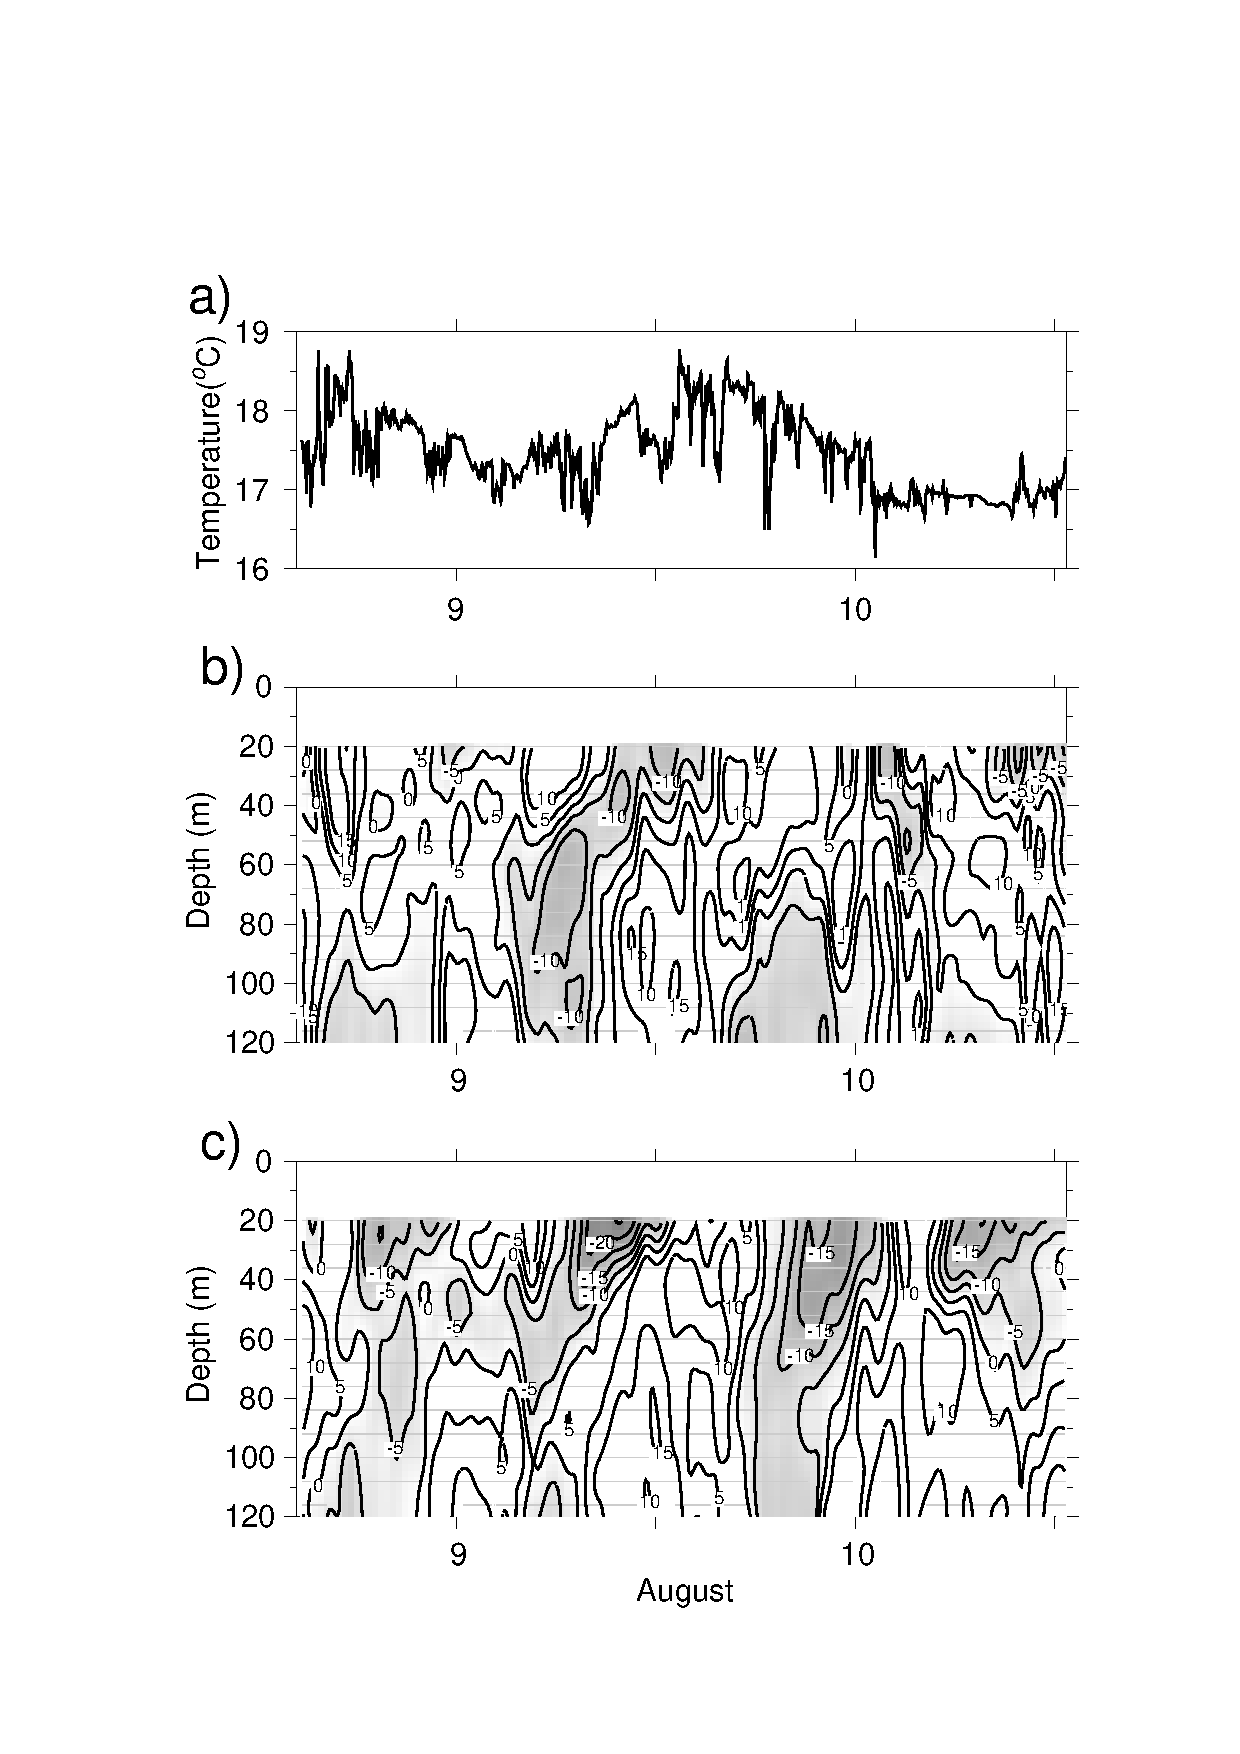
\includegraphics[width=9cm]{adcpph2}%
\caption{(a) Surface temperature (b) east-west and (c) north-south
components of ADCP velocity during the shelf time series
experiment}%
\label{fig:cd114adcpph2}%
\end{figure}

The drift experiment was followed by a 2-day time series station
(Phase 2) at a site in 140m depth where the local bathymetry was
oriented almost exactly north-south. Wind was minimal at the start
of the station and the small net fluxes over the two days there
were shoreward and poleward (Fig~\ref{fig:cd114adcpph2}),
indicative of a relaxation. Variability was dominated by the
internal tides. The semidiurnal barotropic current had an
amplitude of about 4\velc, which was smaller than the amplitude of
the shear in the internal tide, about 10\velc\, between the upper
and lower layers. However, during the series, wind increased
sufficiently southward to produce an average upper layer
equatorward flow above deeper poleward flow. A slight decreasing
trend in surface temperature was consistent with weak renewal of
upwelling. Mean current profiles for both the shelf drift and time
series station indicate upper layer equatorward flow over poleward
flowing bottom boundary layer (Fig.~\ref{fig:cd114meancurr}). U
component was zero or weak onshore.
\begin{figure}
\centering %
\subfigure[]{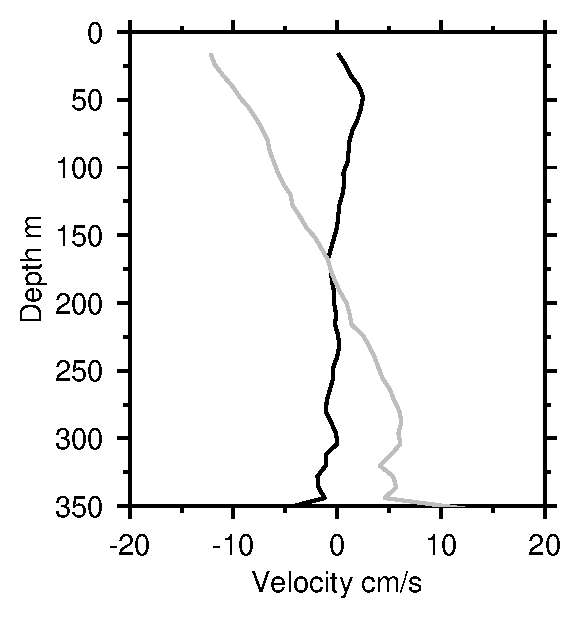
\includegraphics[width=5cm]{meancurrshelf}}%
\subfigure[]{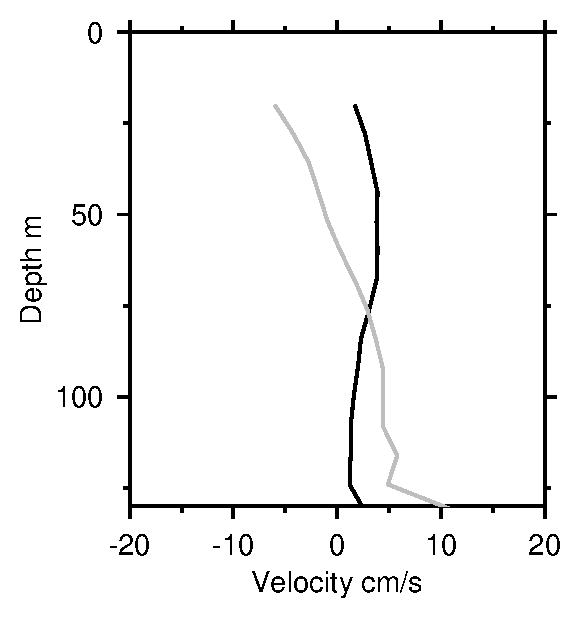
\includegraphics[width=5cm]{meantidal}}%
\caption{Mean current profiles for U (black) and V (grey)
components during, (a) shelf drift and (b) shelf time series
experiment. Standard deviation were consistently less than 0.1
\vel\, below 50m.}
\label{fig:cd114meancurr}%
\end{figure}

\subsection{The filament experiment Leg 2}
\subsubsection{The drifters and water column structure}
\begin{figure}
\centering \arribacap%
\subfigure[]{

\includegraphics[width=7cm]{filam_drf}}%
\subfigure[]{
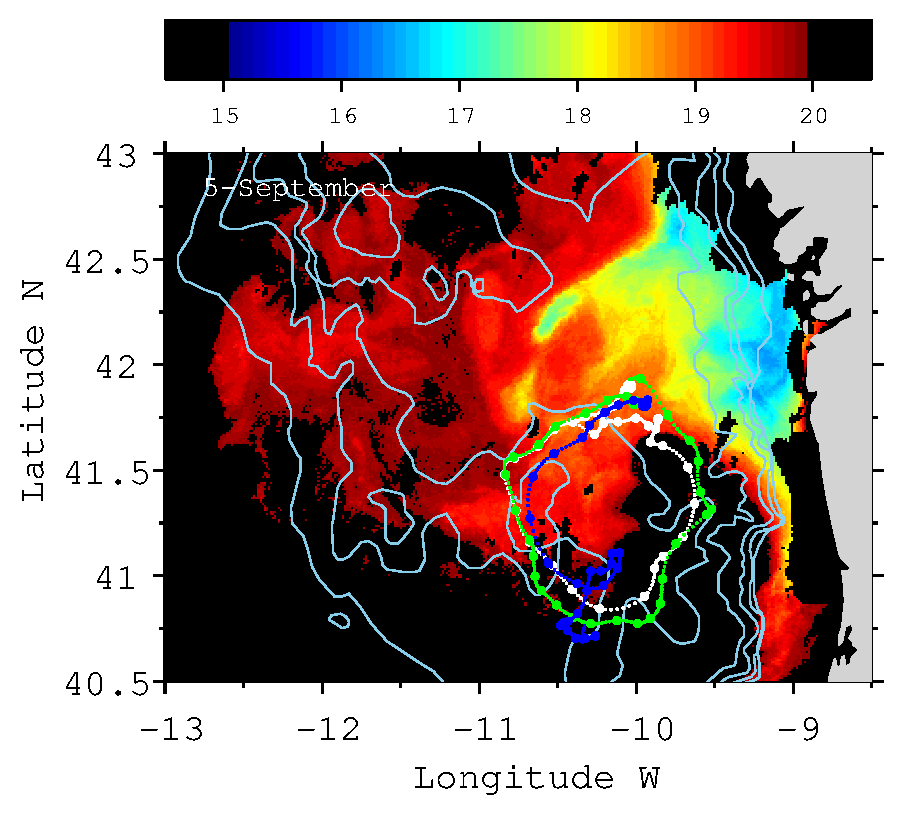
\includegraphics[width=7cm]{eddy}}%
\caption{SST images with drifters overlaid on a) 23 August 1998
with first ten days of deployment overlaid and b) 5 September 1998
with 25 days of drifter data. Dots correspond to the start of each
day.}
\label{fig:cd114drf_sat}%
\end{figure}
Mixed-layer drifters were deployed near the southern core of the
filament (Fig.~\ref{fig:cd114leg2}b) during the weakening of the
winds on 14 August. As the wind continued to decrease in strength
from 10 to 3\vel\, during the next two days, they moved slowly
offshore (0.05\vel) and converged towards the filament's southern
boundary (SB). The convergence rate, calculated following
\citet{Brink91b}, was consistent with a localised sinking at the
SB of about 10md$^{-1}$. Following the wind intensification to
10\vel\, on 17-18 August the northern two accelerated before the
others. One northern drifter traced the offshore extent of the
filament's northern boundary (NB) with mean speed 0.28\vel\,
(Fig.~\ref{fig:cd114drf_sat}a) while the others, which had crossed
the SB, re-circulated shoreward with average speed 0.17\vel\, in
an apparent return flow. It took them another 20 days to complete
the gyre and return close to the launch site
(Fig.~\ref{fig:cd114drf_sat}b). The MLD in the centre of the buoy
array was initially 25m and decreasing
(Fig.~\ref{fig:cd114driftctd}), but deepened to near 50m as the
array drifted towards the SB. The boundary was marked by the
decrease in the salinity maxima at 50-100m, a weak surface minimum
of temperature and density, and the maximum MLD.
\begin{figure} \centering
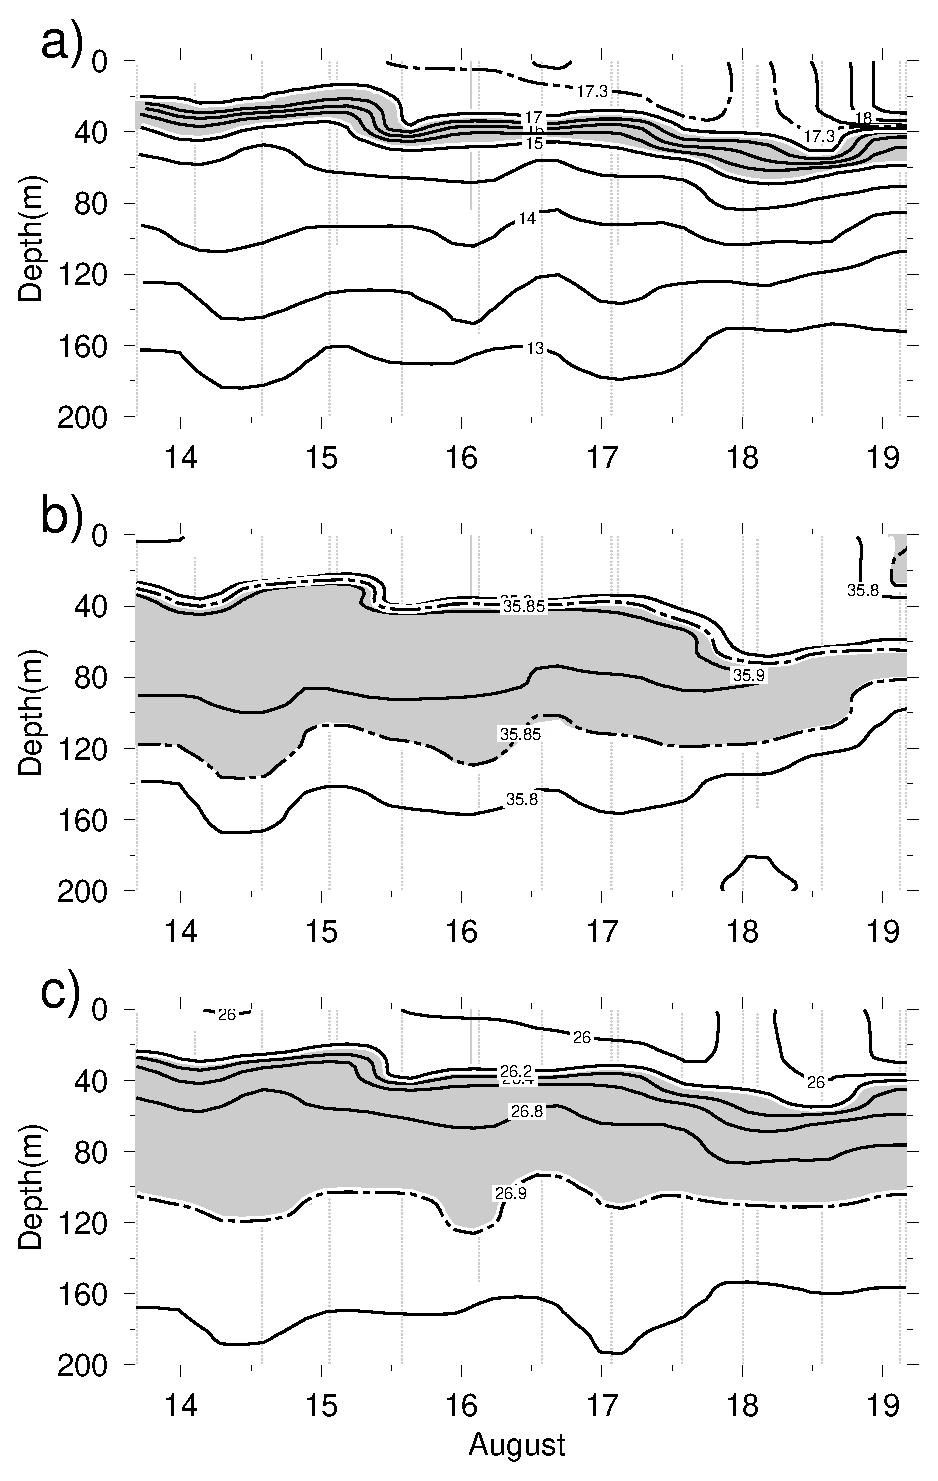
\includegraphics[width=9cm]{driftctd}%
\caption{(a) Temperature (b) salinity and (c) density from the CTD
time series following the filament drifting productivity buoy.}%
\label{fig:cd114driftctd}%
\end{figure}
\subsubsection{Filament cross sections}

\begin{figure}
\centering %
\subfigure[]{\includegraphics[width=6cm]{filam1u}}
\subfigure[]{\includegraphics[width=6cm]{filam1v}} \caption{ Cross
section of the north front a) along filament and b) across
filament velocity structure} \label{fig:cd114fil1vel}
\end{figure}
Several incomplete crossings of Filament A were undertaken during
Leg 2 of CD114 with CTD, ADCP and FLY although not simultaneously.
The first crossing (11-12 August) was done only with underway
measurements following a period of slack winds
(Fig.~\ref{fig:cd114winds}). The ADCP  velocities rotated along
and across filament for the north front are presented in
Fig.~\ref{fig:cd114fil1vel}. Offshore flowing velocities in excess
of 20\velc\,  were measured on the seaward side of the filament
while onshore flow occupied most of the interior of the filament.
Across filament velocities (Fig.~\ref{fig:cd114fil1vel}b) showed
subsurface convergence, particularly below 80m. Unexpectedly,
little baroclinicity was associated with the along filament
component.

\begin{figure}
\begin{widefig}{-.5cm}{-.5cm}
\centering %
\subfigure[]{
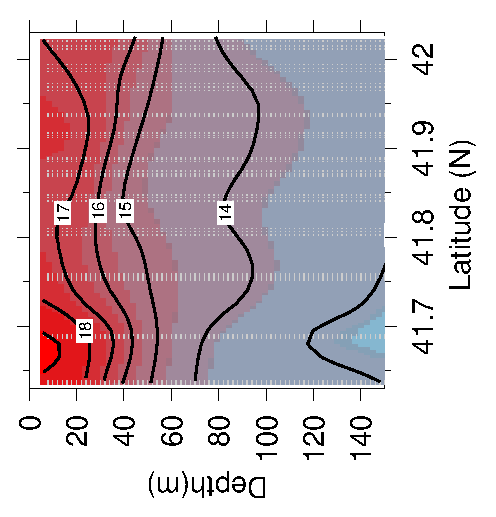
\includegraphics[width=5cm,angle=-90,origin=c]{tempf1}}%
\subfigure[]{
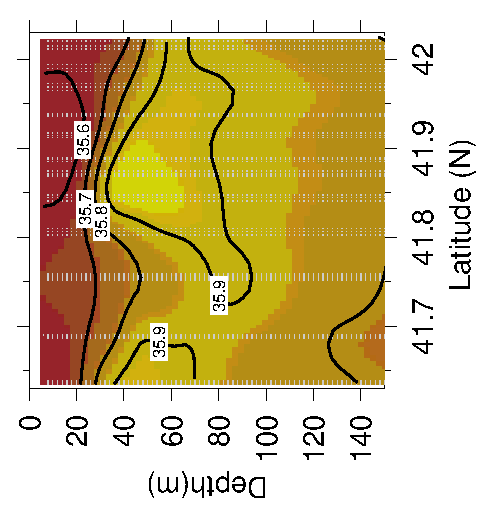
\includegraphics[width=5cm,angle=-90,origin=c]{salf1}}%
\subfigure[]{
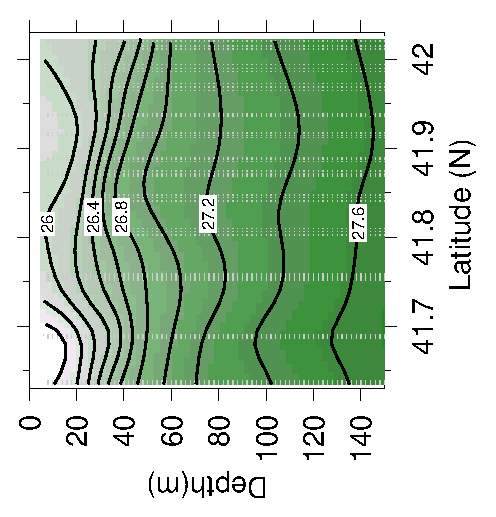
\includegraphics[width=5cm,angle=-90,origin=c]{densf1}}\quad
\subfigure[]{
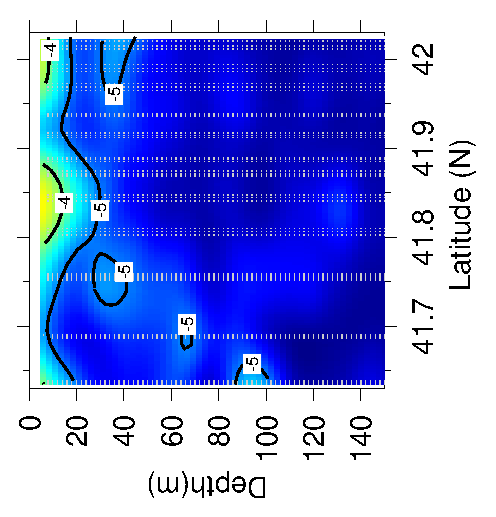
\includegraphics[width=5cm,angle=-90,origin=c]{mixf1}}%
\subfigure[]{\includegraphics[width=5cm]{filam35u}}%
\subfigure[]{\includegraphics[width=5cm]{filam35v}}%
\caption{ Partial cross section of filament of a) temperature, b)
salinity, c) density, e) log dissipation rate f) along filament
and g) across filament velocity structure.}
\label{fig:cd114fil1sec}
\end{widefig}
\end{figure}

The first section sampled with ADCP in conjunction with the FLY
(Fig.~\ref{fig:cd114fil1sec}) on the 16-17 August show details of
the filament interior and the southern front. The southern front
had a shallow frontal structure with isotherms rising and
outcropping from 20m (Fig.~\ref{fig:cd114fil1sec}d), and
isohalines locally deepening in what could be related with
subduction processes. On the filament side of the front, the
isotherms domed above 60m depth, but deepened below. Within the
filament, a salinity maximum was located at this depth. Its
salinity of  $>35.9$psu was closer to oceanic values than to those
of upwelled waters. Surface salinity values $<$35.7 were
restricted to the top 20m at the southern front deepening
northwards to 40m. Enhanced mixing, as represented by the
logarithm of the dissipation rate (Fig.~\ref{fig:cd114fil1sec}d),
was restricted to the top 30m north of the southern front and
shallower than 15m everywhere else, falling to less than $10^{-5}
\mathrm{Wm^{-2}}$ at deeper levels. Little structure is evident in
the velocity section (Fig.~\ref{fig:cd114fil1sec}e-f) except for
strong horizontal shear at the front but with little indication of
convergence compared to Fig.~\ref{fig:cd114fil1vel}b.

\begin{figure}[t]
\begin{widefig}{-1cm}{-1cm}
\centering %
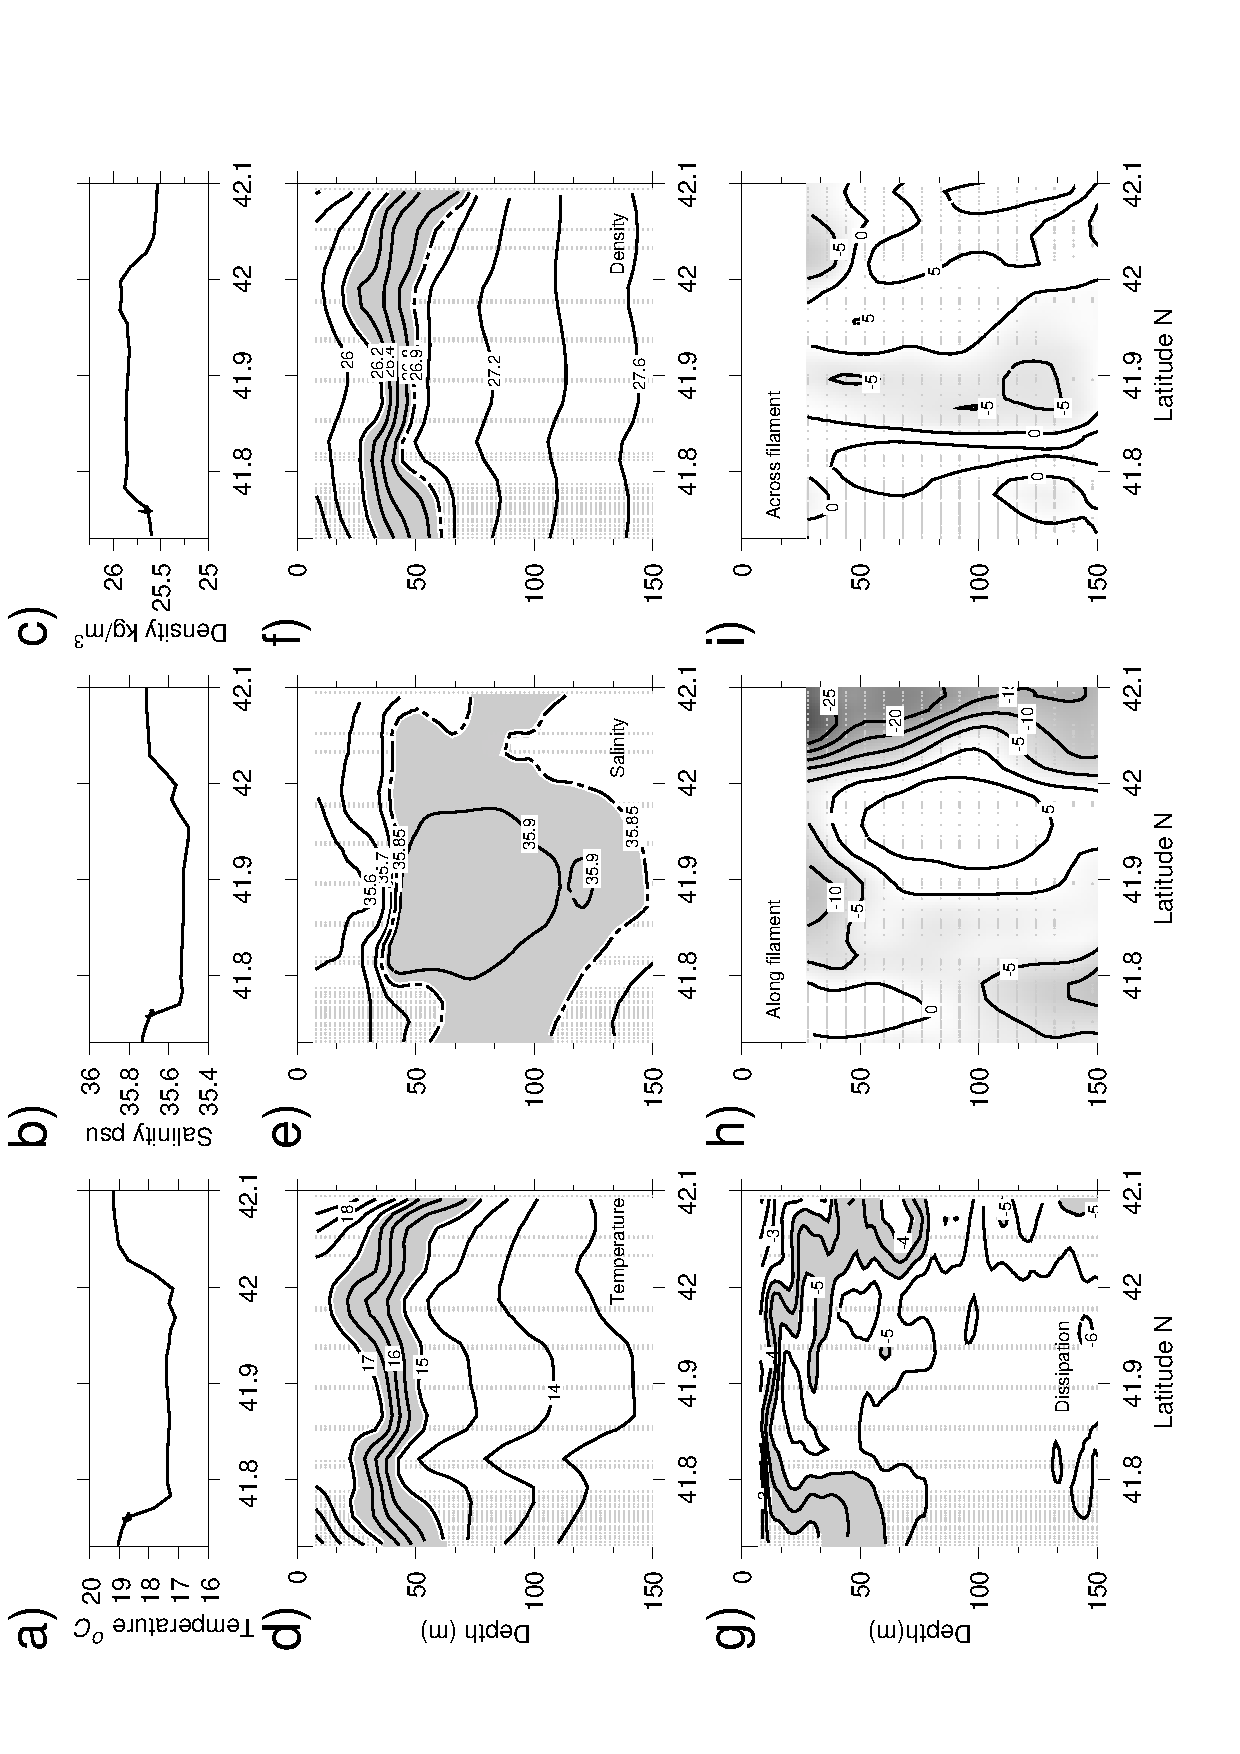
\includegraphics[width=12cm,angle=-90]{section2}%
\caption{Distribution of properties along section 2 across the
filament. Sea surface profiles of (a) temperature (b) salinity and
(c) density. Vertical sections of (d) temperature (e) salinity (f)
density, (g) $\log_{10}$ dissipation rate , (h) along and (i)
across filament velocity. Note onshore flow beneath the centre of
the
filament and weak convergence to its southern side.}%
\label{fig:cd114section2}%
\end{widefig}
\end{figure}
A complete FLY crossing of the filament was undertaken when the
wind speed was increasing on 17-18 August (section 2 in
Fig.~\ref{fig:cd114leg2}a). The surface signal of both frontal
boundaries was clearly seen in temperature, salinity and density
(Fig.~\ref{fig:cd114section2}a-c). Both temperature and salinity
were lowest in the filament core ($<$17.5\deg C, $<$ 35.55psu) and
increased away from the core by up to 2\deg C and 0.2psu in sharp
($<$4km) frontal boundaries. The associated temperature and
density gradients were very similar in both fronts, less than
0.7\deg C $\mathrm{km^{-1}}$ and 0.06 $\mathrm{kg m^{-3}
km^{-1}}$. The filament presented a double core structure
resulting from its merger during Leg 1 of the cruise with the
filament originating at 41.5\deg N, as reported by
\citet{Smyth01}. The temperature, salinity and density fields in
Fig.~\ref{fig:cd114section2}d-f show the double core structure as
two separate domes evident down to 200m. The section did not
continue far enough to sample the full extent of the frontal
regions but they seem restricted to the top 60m. The pycnocline
was situated around 40m, deepening at the fronts, particularly the
northern one, in relation to the stronger baroclinicity seen there
in the velocity data. At the core of the filament, water below 50
m was characterised by a salinity maximum ($>$35.9psu) that did
not extend across the fronts. Fig.~\ref{fig:cd114section2}h and i
shows the velocity structure through the filament rotated into
along and across filament components. The first available ADCP bin
(25m) showed intensification of offshore flow at the filament
boundaries, with larger values at the northern boundary
($>$0.35\vel ) than at the southern one ($\sim$0.1\vel ). The
horizontal shear associated with the fronts was also higher in the
north, $0.5f$ compared to $0.15f$ for the SB ($f\sim 9.7 \times
10^{-5}s^{-1}$). Flow within the filament itself was generally
very weak and, remarkably, directed offshore only in the top 50m;
below there it was weak (0.05-0.1\vel ) and onshore. Near the
fronts, the flow was offshore down to the maximum penetration of
the ADCP with a surface intensified jet showing stronger
baroclinity in the north than in the south.  The total offshore
volume transport calculated in the section was only 0.5Sv, less
than reported for filaments in other regions, though offshore flow
extended beyond the northern limit of the section and may be
underestimated slightly.
\begin{figure}
\centering %
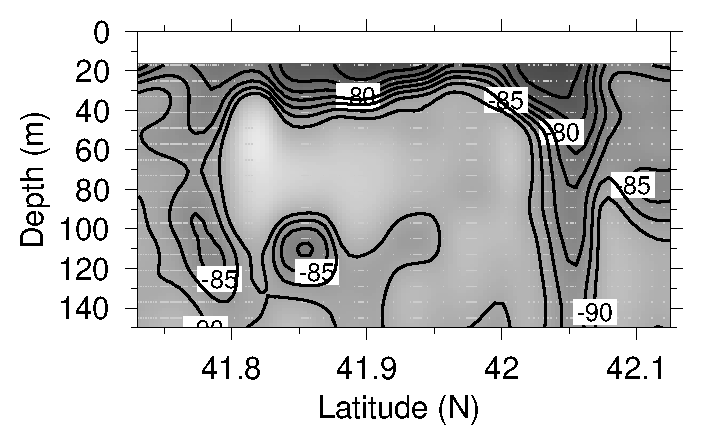
\includegraphics[width=10cm]{filamsv}%
\caption{Distribution of Acoustic Backscatter Intensity in dB
across the filament as derived from the NB ADCP.}
\label{fig:cd114sv}
\end{figure}

Acoustic backscatter intensity (ABI) derived from the ADCP yielded
further support to the property distribution within the filament
(Fig.~\ref{fig:cd114sv}). The ABI is a by-product of the ADCP
which has been successfully related to the abundance of
zooplankton \citep{Flagg89, Zimmerman99}. No attempt was made to
relate ABI data to zooplankton abundance for CD114 cruise although
it is assumed to correlate with abundance of scatterers. ABI
values were derived from the Automatic Gain Control recorded by
the ADCP following \citet{RDI98} as:
\begin{equation}\label{eq:abi}
  ABI=10\log _{10}\left[\frac{4.47\times10^{-20}K_2 K_s (T_x +273)
  (10^{K_c(E-E_r)/10}-1)R^2}{c P K_1 10^{-2\alpha R/10}}\right],
\end{equation}
where $K_2$ is the system noise factor (dimensionless); $K_s$ is a
system constant (dimensionless); $T_x$ is the temperature of the
transducer in \deg C; $K_c$ is the conversion factor for AGC echo
intensity (dB/count); $E$ is the AGC echo intensity (counts);
$E_r$ s the real-time reference level for AGC echo intensity
(counts); $R$ is range along beam to scatterers (m);$c$ is sound
speed (m/s); $P$ is transmit pulse length (m); $K_1$ is real-time
power into the water (W); and $\alpha$ is the absorption
coefficient of water (dB/m). Higher ABI reflecting larger amounts
of scatterers are clearly visible at both fronts and in the
surface layer, while minimum levels were recorded in the core in
the region of the salinity maximum. High ABI values penetrated
deeper at the northern boundary than at the southern one
reflecting the larger intensity of the first.
\begin{figure}
\begin{widefig}{-.7cm}{-.7cm}
\centering \subfigure[]{
\includegraphics[width=5cm,angle=-90,origin=c]{southtemp}}%
\subfigure[]{
\includegraphics[width=5cm,angle=-90,origin=c]{southsal}}%
\subfigure[]{
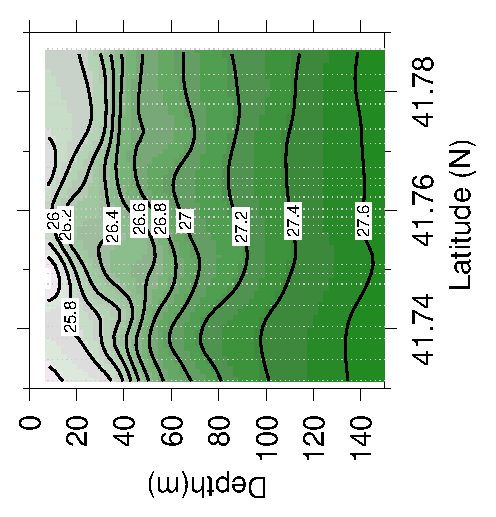
\includegraphics[width=5cm,angle=-90,origin=c]{southdens}}\quad%
\subfigure[]{
\includegraphics[width=5cm,angle=-90,origin=c]{southmix}}%
\subfigure[]{\includegraphics[trim= 0 5 0 0,clip,width=5cm]{flysouthu}}%
\subfigure[]{
\includegraphics[trim= 0 5 0 0,clip,width=5cm]{flysouthv}}
\caption{ Distribution of properties in detailed sections of the
filament's south front of a) temperature, b) salinity, c) density,
e) log dissipation rate f) along filament and g) across filament
velocity structure} \label{fig:cd114southfsec}
\end{widefig}\end{figure}

A blown up section of measurements within the southern front
(Fig.~\ref{fig:cd114southfsec}) clearly shows indications of
subduction at the front. A lower temperature, vertically mixed
lens 2km wide (Fig.~\ref{fig:cd114southfsec}a) was associated with
a low salinity intrusion (Fig.~\ref{fig:cd114southfsec}b) and
locally enhanced mixing (Fig.~\ref{fig:cd114southfsec}d, with
values larger than $10^{-4} \mathrm{W m^{-2}}$). Strong mixing was
also measured down to 40m depth in the frontal region immediately
south of the intrusion where the isotherms outcrop to the surface.
The velocity structure was weak and complex. Flow was locally
onshore at the intrusion but mostly offshore south and north of it
(Fig.~\ref{fig:cd114southfsec}e). The across filament component
was very patchy with weak convergence at the intrusion from 40m
depth to the uppermost ADCP bin at 28m
(Fig.~\ref{fig:cd114southfsec}f).

\subsubsection{Water masses}
\begin{figure}
\centering %
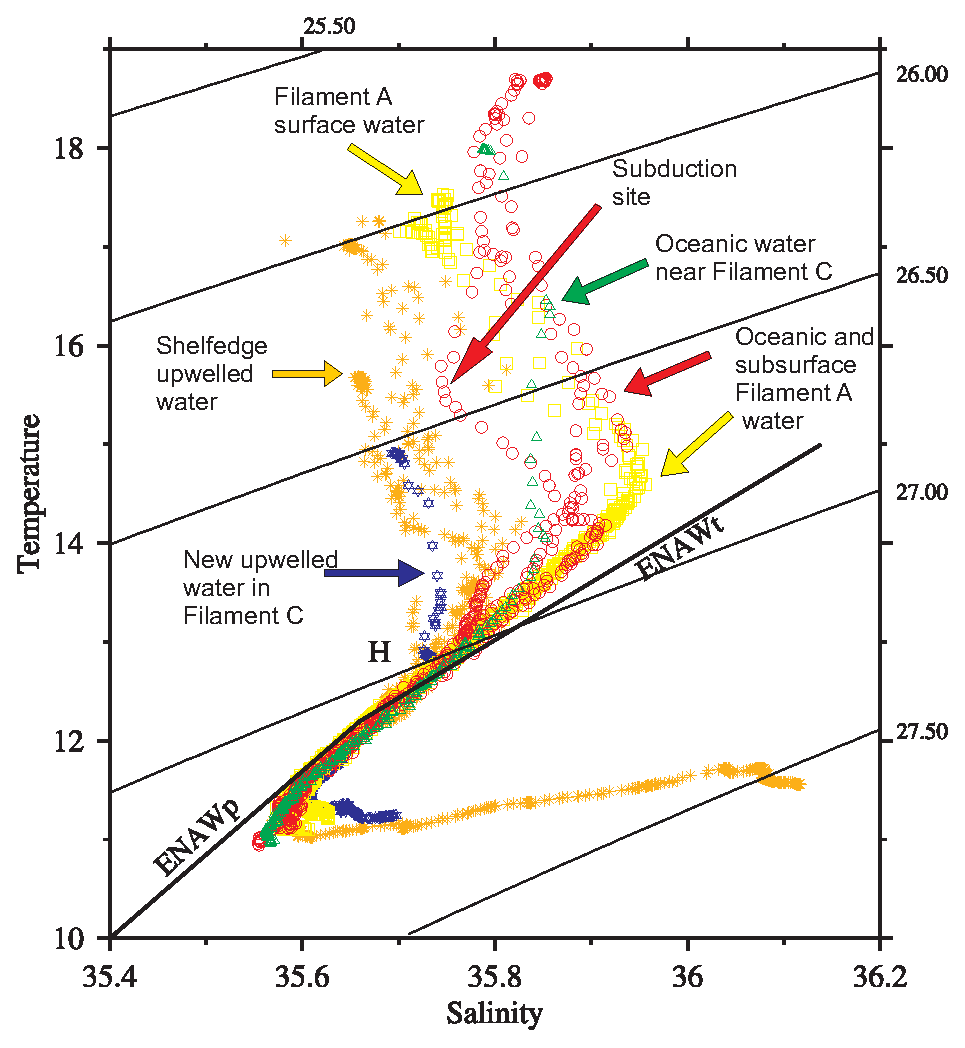
\includegraphics[width=7cm]{TSdiag}%
\caption{T/S plot of selected CTD stations showing the different
water masses in filaments A and C. See text for details.}
\label{fig:cd114ts}
\end{figure}
The AVHRR image (Fig.~\ref{fig:cd114leg2}) gives no indication of
whether Filament A was a superficial or a substantive
oceanographic feature. However, a T/S diagram of selected CTD
casts during the cruise (Fig.~\ref{fig:cd114ts}) provides evidence
that it was surprisingly shallow, and that the only part that
comprised water that had upwelled on the shelf was in the surface
layers. These layers had a salinity of $\sim$35.74psu, indicating
an origin at about 180m depth. Their temperature, 1-1.5\deg C less
than that of surrounding oceanic surface waters, suggests that
there had been considerable warming of the upwelled water as it
was advected offshore.  The mid-depth filament waters (yellow in
Fig.~\ref{fig:cd114ts}), on the other hand, had a signature that
was closer to the surrounding sub-surface oceanic water (red) than
the upwelled shelf water (orange). This interpretation is
consistent with the observed along-filament flow
(Fig.~\ref{fig:cd114section2}) where oceanic water was carried
shoreward beneath a superficial offshore moving filament
structure. A single CTD profile made on the filament's southern
boundary (red, and marked ``Subduction site'') had T/S
characteristics that lay between those of the upwelled water and
the truly oceanic stations. At, and just beneath, the surface its
properties were oceanic, but below 20m there was a salinity
minimum which had the same value as that of the upwelled water in
the surface layer of the filament.  This suggests subduction in
the convergence zone, as indicated by the drifter tracks
(Fig.~\ref{fig:cd114leg2}).  The situation in the actively growing
filament C, which started developing close to Finisterre after 13
August (described in more detail by \citet{Smyth01}) contrasted
with that of the weakening filament A. Throughout its depth range
filament C was composed of of colder, newly upwelled water (blue)
moving offshore.

\subsubsection{Turbulence observations}
Only few observations of turbulent dissipation in filament
structures have been made.  In a 100km wide eddy-like feature off
Oregon, \citet{Moum88} found very low dissipation levels ($<
10^{-5} W m^{-2}$) in the core but enhanced values in regions of
high shear at the edge of the structure and in an intrusion into
the core. Generally low dissipation levels were observed below the
surface layer in some upwelling filaments off California
\citep{Dewey93}, apart from the core of a narrow (10km wide)
filament, where locally enhanced values of order $10^{-3} W
m^{-2}$ were observed.

Enhanced mixing was observed in both fronts
(Fig.~\ref{fig:cd114section2}g) although larger integrated values
were found on the northern boundary. In the filament core, active
mixing was restricted to the surface 15m, while in the fronts,
high values of TKE penetrated to 80m in the NB and 60m in the SB.
Representative values of integrated TKE and derived $K_z$ for the
thermocline are presented in Table~\ref{tb:cd114mixing}.
Confidence intervals for the estimates were calculated using a
non-parametric (bootstrap) method \citep{Press92}. The thermocline
was subjectively chosen to be 15-17\deg C, and total dissipation
was integrated over the depth of the dissipation profiles
(typically 250 m). $K_z$ estimates spanned three orders of
magnitude across the filament. Estimated errors were similar to
those for the shelf experiment, albeit with less confidence since
they are based on fewer observations (typically 10 profiles). The
enhanced localised mixing in the thermocline of the SB is believed
to be related to the subduction processes. Selected 5 drops
averaged $K_z$ profiles (Fig.~\ref{fig:cd114flydrops}) exemplify
the differences encountered in the filament. A broad layer of 30m
of high diffusivity was present in the southern front at the
intrusion (Fig.~\ref{fig:cd114flydrops}a). The highest
diffusivities were measured there due to the weak stratification
of the intrusion, rapidly falling to levels similar to the
filament core, an order of magnitude smaller
(Fig.~\ref{fig:cd114flydrops}b). In the northern front,
diffusivities of value $\sim$3\mixc were measured near the surface
and at the pycnocline falling to the filament core levels in
between (Fig.~\ref{fig:cd114flydrops}c).

\begin{figure}
\centering %
\subfigure[]{\includegraphics[width=5cm]{southkz}}%
\subfigure[]{\includegraphics[width=5cm]{middle}}%
\subfigure[]{\includegraphics[width=5cm]{northkz}}%
\caption{Examples of averaged $K_z$ profile estimates at the south
and north fronts and the filament interior. Five consecutive FLY
drops were used in the calculations.} \label{fig:cd114flydrops}
\end{figure}
\begin{table}[h]
  \centering
\begin{tabular}{ccccc}
 & $K_z$  & 75\% confidence & Thermocline  & Total dissipation  \\
 & $\mathrm{cm^2 s^{-1}}$  &  limits $\mathrm{cm^2 s^{-1}}$ &
 dissipation $\mathrm{W m^{-2}}$  & $\mathrm{W m^{-2}}$ \\
\hline \hline
South Front & 1.6 & 1.1 & 4 $10^{-3}$ & 8.5 $10^{-3}$  \\
Core & 0.015 & 0.01  & 0.3 $10^{-3}$ & 1.4 $10^{-3}$ \\
  North Front & 0.1 & 0.04 & 1.5 $10^{-3}$ & 12.6 $10^{-3}$ \\
\hline \hline
\end{tabular}  \caption{Vertical eddy diffusivity and vertically integrated
dissipation rates for the filament survey. }\label{tb:cd114mixing}
\end{table}

\section{Discussion}
Both periods of sampling took place when winds were changing from
strongly upwelling favourable to near zero, but winds were never
actually downwelling favourable. The experiments are therefore
representative of relaxation following an upwelling event.  In
this respect, results seem typical in the indications of
convergence at the filament boundary, as also observed by
\citet{Flament85} and \citet{Flament00} off California, the
establishment of poleward flow on the shelf and slope, like
California \citep{Winant87}, and the general decrease in extent of
the filaments with weakening wind, previously noted off Iberia by
\citet{Haynes93}. Indications of persistent poleward undercurrent
during the summer in the Galician system were seen in
current-meter records of 1989 at 280m depth in 300m of water
\citep{Huthnance02}, reversing briefly only during the strongest
upwelling wind events. They also encountered predominant poleward
flow over the slope from May to September 1999 at 430m depth.
During the wind relaxation of Leg 1, the poleward undercurrent
became shallower, reaching depths of 170m over the slope
(Fig.~\ref{fig:cd114adcpleg1}), and depth-integrated transport
reversed to poleward. Across-shelf transport also changed
accordingly; seaward at the beginning of drift but onshore on the
last day and during Phase 2. The decreasing contribution to the
filament seen during the shelf experiment and the relatively small
offshore filament transport - compared to 1-3 SV in active
filaments off California \citep{Strub91} and NW Africa
\citep{Barton98} - reflect the weakening system.  However, both
drift experiments sampled packets of water recently upwelled and
represent conditions commonly found in the highly variable system
off Galicia.

There was considerable spatial variability in the observations of
diffusion in the filament.  On its southern boundary the levels
were similar to those observed at the shelf edge (about 1\mixc,
\citet{Barton01}), whilst on its northern boundary they were an
order of magnitude smaller. Very low values were observed within
the core of the filament (about 0.01\mixc ).  This distribution of
vertical mixing is closer to that observed in the wide eddy like
structure off Oregon, \citep{Moum88} than the narrow filament off
California \citep{Dewey93}.  It is not possible to give a specific
explanation for these differences from the observations made in
the filament, but it is clear that the enhanced diffusion
coefficients occurred in regions of high vertical shear. Both
frontal regions showed similar surface gradients and horizontal
extend in contrast with previous measurements that showed
consistently sharper fronts in the cyclonic boundary (our southern
front) of filaments \citep{Washburn91,Dewey91,Flament00}.  Sharp
convergent shear fronts associated with upwelling filaments have
been reported by several authors \citep[e.g.][]{Moum90,Flament00}.
In the present experiment, ADCP data showed inconclusive evidences
of weak convergence in both boundaries but was supported by the
observed convergence of the drifters towards the southern
boundary. \citet{Flament00} found subducting layers during slack
winds in a cyclonic convergence front. The author suggested a
secondary frictional flow induced by the along-front geostrophic
flow as the possible cause of the convergence. The subducting
layer found in the southern front was of similar size than the one
sampled by \citet{Flament00} but the associated frontal shears
were far weaker. No information on the along filament extend of
the subducting layer was gathered but it might have been very
localised, associated with the curvature of the front causing
along-filament convergence rather than across-filament
\citep{Shearman99}.

A vertical mixing time, $\tau$, across a thermocline of thickness
h, should approximate to $\tau = {h^2}/{K_z}$, on dimensional
grounds. If $h$ is (say) 20m then $\tau$ will increase from about
1 month to 1 year as $\mathrm{K_z}$ decreases from 1 to 0.1\mixc.
On the shelf a rate of 1\mixc would be large enough to cause the
thermocline to both broaden and transport material into the lower
layers over the duration of summer. However, in the lifetime of a
filament (order 1 week) vertical mixing makes only a small
contribution to the evolution of the temperature and nutrient
structure.  Any observed changes must be due to other horizontally
dominated factors, such as eddies.  At the southern boundary,
convergence appears to dominate vertical mixing, causing sinking
at about 10$\mathrm{m day^{-1}}$ ($\tau=7$ days when $h$ = 10m and
$\mathrm{K_z}$ = 1.6\mixc ).  Water mass characteristics within
the filament will not be significantly modified by vertical mixing
during its lifetime, though surface warming and horizontal
exchanges will gradually change them.

The apparently anomalous double core structure of filament A may
result from several factors. It was one of the ``oldest''
filaments, having developed at the start of the upwelling season,
and had therefore been subject to several cycles of development
and relaxation prior to sampling. Moreover, it had merged with a
second filament (B) arising some distance to the south.  The
shoreward flow in its centre was probably a relic of the
recirculation between the originally separate filaments A and B.
Finally, it was sampled during a period of minimal wind, when the
slow drifter speeds and convergence indicate relaxation of the
system, so that its structure may not be typical of an active
filament.  In this respect, filament C may have been more
representative, but developed too late to be thoroughly sampled.
The presence of shoreward flow beneath the surface signature of
the merged filaments underlines the difficulty of making transport
estimates solely on the basis of remotely sensed sea surface
temperatures. Finally, the results show that there is not a simple
one way transport from shelf to open ocean or sub-surface to
surface. Three of the four filament deployed drifters recirculated
shoreward.  Their trajectories suggests that at least some waters
transported offshore in the filament may return to near slope on a
time scale of a month. However, it must be remembered that the
behaviour of surface drifters where they crossed the convergence
zone on the filament boundary is not truly Lagrangian in that they
cannot follow submerging water parcels. The evidence of subduction
at the southern boundary of the filament implies vertical
recirculation of water parcels on a relatively short time scale.
Given the typically 2 weeks cycling of wind forcing observed here,
these vertical exchanges may have implications on significant
biological time scales.
\begin{figure}
\centering \arribacap%
\subfigure[]{
\includegraphics[width=7cm]{15sepdrifters}}%
\subfigure[]{
\includegraphics[height=6.5cm]{7sep95}}%
\caption{SST images on a) 15 September 1998 overlaid with drifters
positions five days either side of image date
 and b) 7 September 1995. White dots
correspond to the start of each day. Clouds are masked black.}
\label{fig:cd114_satend}%
\end{figure}

The disappearance of Filament A in September was brought about by
the sudden weakening of the upwelling favourable winds as seen in
Fig.~\ref{fig:cd114upidx}. During that time, \citet{Peliz02}
measured the establishment of off the shelf poleward flow.
Filament A drifted northwards (Fig.~\ref{fig:cd114sst}h-i)
advected by a warm tongue anomaly reminiscent of the winter slope
poleward flow \citep[e.g.][]{Haynes90}. Filament A weakened and
became narrower (Fig.~\ref{fig:cd114_satend}a). The offshore end
of the filament bent southwards and the frontal boundaries became
less well defined, probably as a result of increase insulation due
to the slackening of the winds. The poleward anomaly strengthened
and the one drifter that was within its influence moved northwards
with larger speed than the other three. A similar situation, also
involving the 42\deg N filament, was identified in SST imagery in
1995 (Fig.~\ref{fig:cd114_satend}b). The offshore filament end is
broad, badly defined and bents southward while a warm anomaly
develops over the slope. At the coast, another warm anomaly is
clearly visible extending over 150km. It has been related to a
poleward coastal countercurrent which is typical at the end of the
upwelling regime \citep{Sordo01}. In the absence of upwelling
favourable winds, the meridional density gradient quickly forces
the poleward flow over the slope and filaments are slowly cut off
from its water source over the shelf. With time, their surface
signal disappears masked by solar insulation or horizontal mixing.

\section{Conclusions}%
A combination of Lagrangian and other observations has revealed
complex features of the upwelling filament system on and offshore
of the NW Iberian continental shelf.  Observations were made
during a period of upwelling favourable but weakening  winds.
\begin{itemize}
\item On the shelf near the source of the 42\deg N filament, it was found
the net offshore flux to the filament decreased as upwelling
favourable winds relaxed to near zero.  At the same time
alongshore currents reversed to slightly poleward.
\item The 42\deg N filament had an unusual double core structure arising
from the earlier merger of two separate filaments. Remnant return
flow below the surface carried oceanic water shoreward between and
under the two merged filament cores.
\item Offshore transport in the filament was estimated at only 0.5 Sv
moving offshore,  which is small compared to filament transports
reported elsewhere.  This low level of transport is compatible
with measurements made during a weakening of the upwelling and
almost certainly underestimates transport in a developing
filament.
\item Enhanced turbulence was found in the filament boundaries, and
probably results  from stronger baroclinic shear at the northern
boundary ($\mathrm{K_z}$=0.1\mixc ) and possible subduction at the
southern boundary ($\mathrm{K_z}$=1.6\mixc ). Overall vertical
mixing in the filament itself appeared to be small
($\mathrm{K_z}$=0.01\mixc ).
\item Drifters showed some water transported off shelf in the filament
was carried far out to sea, but some could recirculate on a time
scale of a month back to the shelf edge. This has strong
implications for the biology of the region and in particular the
retention of larvae spawned on the shelf.
\end{itemize}
The present observations were obtained in support of a
multi-disciplinary cruise with multiple objectives and because of
sampling compromises are not synoptic but only representative of
restricted areas at specific times. Nevertheless, the data set
provides new information on the behaviour of the filament system
and highlights important questions as to the initiation and decay
of filament structures.
